\documentclass[12pt,a4paper]{article}

\usepackage{amsmath,amssymb}
\usepackage{booktabs}
\usepackage{graphicx}
\usepackage{hyperref}
\usepackage[numbers,sort&compress]{natbib}
\usepackage[margin=1in]{geometry}
\usepackage{float}
\usepackage{url}
\urlstyle{same}
\usepackage{caption}
\usepackage{subcaption}
\usepackage{tabularx}
\usepackage{array}
\usepackage{ragged2e}

\makeatletter
\setlength{\@fptop}{0pt}
\setlength{\@fpsep}{3\baselineskip}
\setlength{\@fpbot}{0pt plus 1fil}
\makeatother

\hypersetup{
    colorlinks=true,
    linkcolor=blue,
    citecolor=blue,
    urlcolor=blue
}

\title{Decisive Shock or Strategic Exhaustion? A Dynamical Model of War Termination Mechanisms}

\author{
  Jake Enholm\\
  Data Scientist
}

\date{\today}

\begin{document}

\maketitle

\begin{abstract}
This paper proposes a framework for separating shock-driven and exhaustion-driven termination mechanisms in armed conflict. We introduce two complementary composite indices---the Decisive Shock Score (DSS) and the Strategic Exhaustion Score (SES)---defined as transparent weighted averages of normalized, dimensionless component scores, and apply them to a dataset of 4,812 wars. Many DSS components require post-hoc information; we therefore distinguish observed DSS (explanatory) from a structural DSS proxy (partially predictive, using only pre-war features). Among the 91 wars with sufficient battle-level data, 2.2\% are classified as decisive shock and 22.0\% as strategic exhaustion; the remainder are uncertain or mixed. A dynamical simulation model demonstrates that shock and exhaustion mechanisms can coexist in a bounded state-space model: when calibrated to seven historical cases, the mechanism classifier agrees with our pre-specified case-study labels in six cases (86\%). We treat this as an internal consistency check, not an independent validation result. A random forest classifier achieves 72.7\% accuracy predicting war duration from material-capability features, suggesting nonlinear structure in these predictors. Independent blind validation of the mechanism classifier remains future work.
\end{abstract}


\section{Introduction}
\label{sec:introduction}
The question of how wars end has occupied strategic thinkers for centuries. Alfred Thayer Mahan's influential treatise on sea power argued that naval supremacy, expressed through decisive fleet engagements, determines the outcomes of wars and shapes the fate of nations \citep{mahan1890}. In this view, the decisive battle is the mechanism through which political objectives are achieved: destroy the enemy's capacity to fight, and the war is won. The opposing view, rooted in Clausewitz's observations and refined by modern scholars of attrition warfare, holds that wars are decided not by single moments of brilliance but by the gradual exhaustion of an adversary's material and human resources \citep{clausewitz1832}. In this framework, decisive battles are rare anomalies; most wars are won by the side that can sustain losses longer.

These two hypotheses, decisive shock versus strategic exhaustion, carry profoundly different implications for military strategy, resource allocation, and foreign policy. If wars are decided by decisive battles, then investment in elite military capabilities and offensive doctrine is warranted. If wars are decided by exhaustion, then industrial capacity, logistics, and political will become the decisive factors. Yet the empirical literature has largely treated this as a binary classification problem: each war is either ``decisive'' or ``attritional,'' with limited attention to the possibility that both mechanisms operate simultaneously at different phases of conflict.

This paper's key contribution is suggesting that decisive events and attritional processes are not competing explanations but interacting mechanisms occurring at different phases of conflict. Attrition changes the state space, degrading military capacity, eroding economic resilience, and undermining political will, and decisive shocks exploit the altered state space. The historical mistake is treating the visible collapse event as the entire cause, when it often operates atop an attritional substrate that has already shifted the strategic balance (Figure~\ref{fig:conceptual}).

\begin{figure}[ht]
\centering
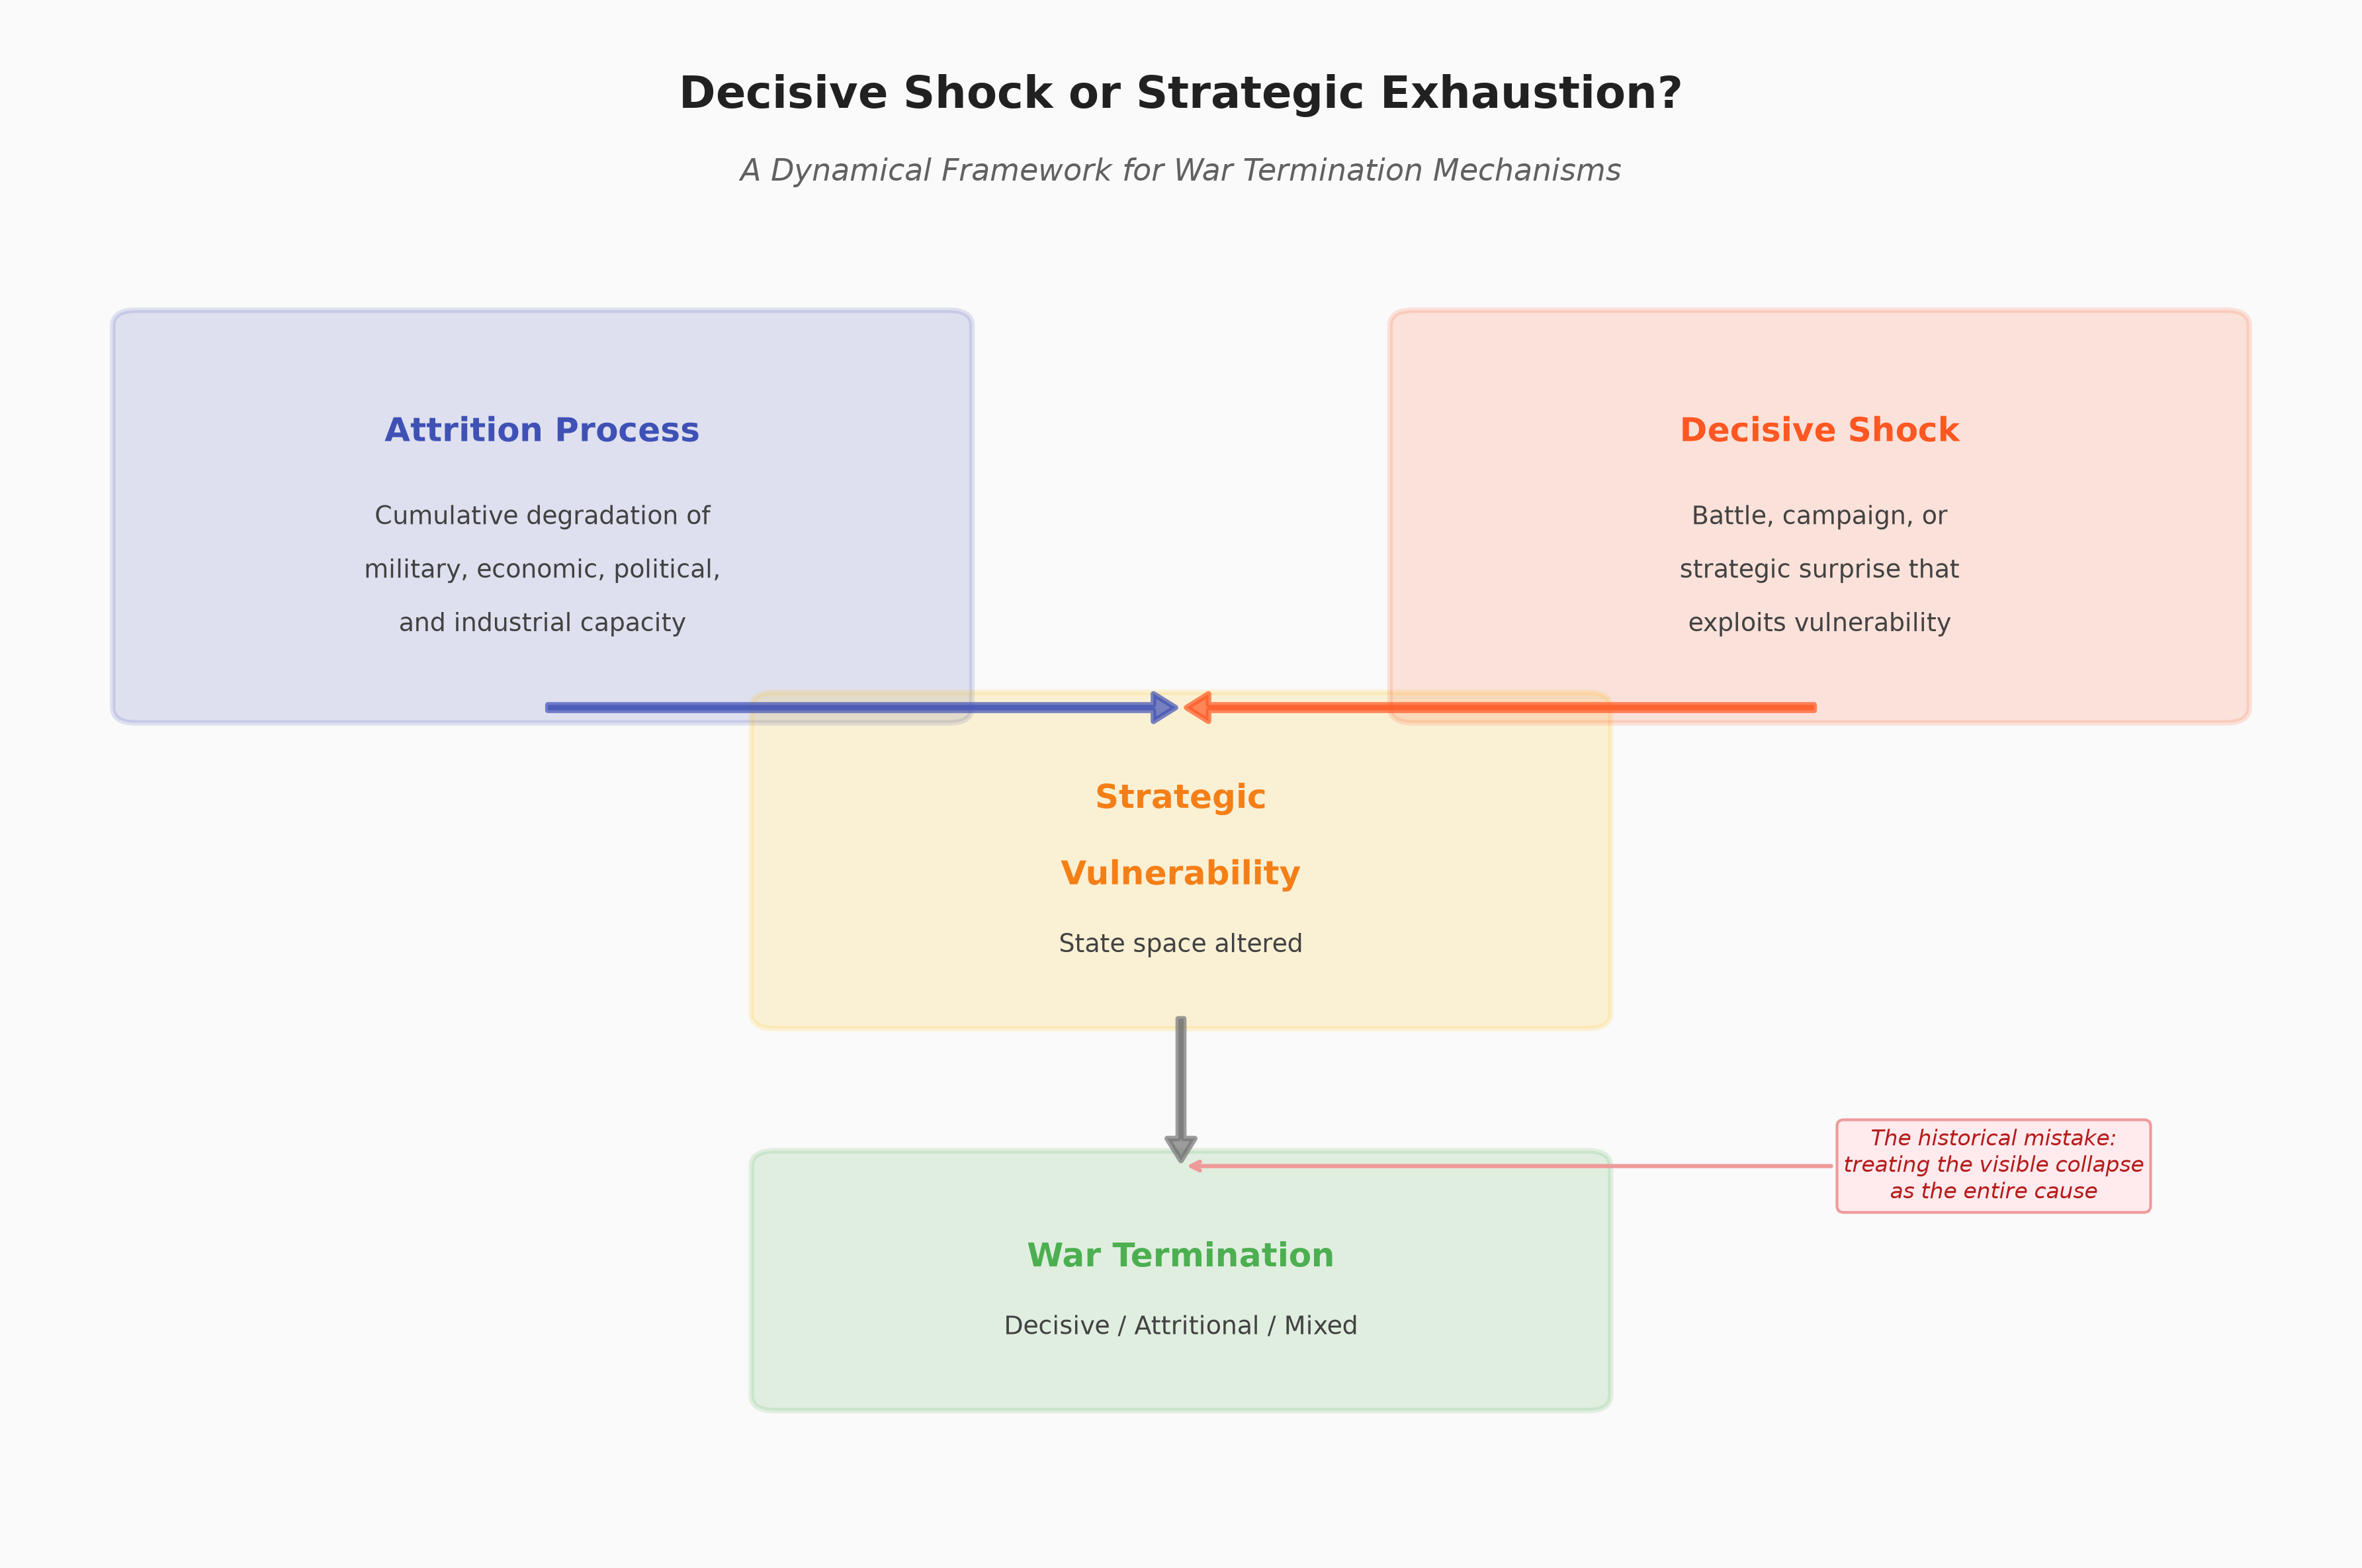
\includegraphics[width=0.8\textwidth]{figures/fig_01_conceptual_model.png}
\caption{Conceptual model of the attritional iceberg. The visible decisive shock operates atop a larger attritional substrate that has already shifted the strategic balance.}
\label{fig:conceptual}
\end{figure}

To test this framework, we develop a computational approach comprising three components: (1) the Decisive Shock Score (DSS), which quantifies the role of decisive battles or campaigns in war outcomes (noting that some DSS components require post-hoc information); (2) the Strategic Exhaustion Score (SES), which measures cumulative attritional dynamics; and (3) a dynamical simulation model that generates synthetic war trajectories under varying parameter regimes. We apply these tools to a comprehensive dataset covering 4,812 wars from antiquity to the modern era, enabling large-n quantitative analysis of war termination mechanisms.

\subsection{What the Model Generates (and What It Does Not)}

The model's classification target is deliberately narrow. It generates:

\begin{itemize}
    \item \textbf{Termination pathway class}: whether a war is more likely to terminate through decisive shock, strategic exhaustion, or a mixed process.
    \item \textbf{Dominance of mechanism}: which mechanism, shock or attrition, dominates at each phase of the conflict.
    \item \textbf{Trajectory shape}: the qualitative pattern of state variable evolution over time.
\end{itemize}

The model does \emph{not} attempt to generate:

\begin{itemize}
    \item The exact winner of a specific conflict.
    \item The date of surrender or ceasefire.
    \item Battlefield-level outcomes or tactical events.
    \item The specific battles that will occur or their timing.
\end{itemize}

This narrow classification target reflects a deliberate scientific choice. Clausewitzian strategic outcomes emerge from many interacting systems: leadership, intelligence, geography, technology, domestic politics, weather, and chance. No parsimonious model can capture all of these. Rather than claiming broad predictive power, we focus on identifying qualitative mechanism classes and the structural conditions under which each dominates.

\subsection{What This Paper Does and Does Not Claim}

\begin{table}[H]
\centering
\small
\setlength{\tabcolsep}{4pt}
\renewcommand{\arraystretch}{1.12}
\caption{Claim scope: what this paper does and does not claim. The distinction between internal model consistency and independent empirical validation is central to interpreting the results.}
\label{tab:scope}
\begin{tabularx}{\textwidth}{@{}
>{\RaggedRight\arraybackslash}p{0.20\textwidth}
>{\RaggedRight\arraybackslash}X
>{\RaggedRight\arraybackslash}X
@{}}
\toprule
\textbf{Claim type} & \textbf{Paper does claim} & \textbf{Paper does not claim} \\
\midrule
DSS/SES & Transparent scoring framework using normalized, dimensionless indices & Ground-truth taxonomy of wars \\
Simulation & Mechanism plausibility demonstration & Precise historical reconstruction \\
Case studies & Calibrated comparison with author-assigned labels & Independent historian validation \\
RF/LR & Duration prediction baseline showing nonlinear structure & Test of DSS/SES superiority \\
Attritional iceberg & Pattern in 91 wars with complete battle-level data & Universal law of war \\
Mechanism classifier & Internal consistency check (6/7 agreement) & Independent predictive accuracy \\
\bottomrule
\end{tabularx}
\end{table}

We find several key results. First, a logistic regression model using ten material-capability features (CINC scores, military expenditure, energy consumption, military personnel, iron and steel production, and their percentage changes) achieves 55.0\% cross-validated accuracy (AUC = 0.551) in predicting war duration category, only 2.7 percentage points above the null baseline of 52.3\%, while a random forest achieves 72.7\% accuracy, demonstrating that nonlinear interactions among material-capability features contain substantial predictive information that linear models cannot capture. Battle deaths are excluded from both models as wartime outcomes, not ex-ante predictors. Second, our mechanism classifier agrees with author-assigned labels in 6 of 7 cases by separating termination events from strategic causes. Third, the simulation provides a mechanistic demonstration that DSS and SES can emerge from interacting attritional and shock processes: when calibrated to historical initial conditions, the model produces trajectory classes consistent with the mechanism-trajectory classifier in 6 of 7 cases. This demonstration is consistent with internal model consistency while also revealing the fundamental difficulty of generating specific historical outcomes with simplified models.

The remainder of this paper is organized as follows. Section~\ref{sec:background} reviews the theoretical literature on war termination. Section~\ref{sec:data} describes our multi-source dataset. Section~\ref{sec:methods} details the DSS, SES, and simulation methodology. Section~\ref{sec:results} presents our empirical findings. Section~\ref{sec:discussion} interprets the results in light of existing theory, and Section~\ref{sec:conclusion} concludes with directions for future research.

\clearpage

\section{Background}
\label{sec:background}
\subsection{The Mahan Hypothesis: Decisive Battle and Sea Power}

Alfred Thayer Mahan's \textit{The Influence of Sea Power upon History, 1660--1783} \citep{mahan1890} established the theoretical foundation for the decisive battle hypothesis. Drawing on Britain's naval dominance in the eighteenth century, Mahan emphasized concentration of naval power, command of maritime communications, and the ability of sea power to influence national strategy as the primary determinants of war outcomes. The decisive battle, in Mahan's framework, is not merely a tactical victory but a strategic mechanism: by destroying the enemy's naval capability in a single engagement, the victorious power secures the conditions for political settlement on favorable terms. Critically, Mahan's analysis extended well beyond fleet engagements to encompass commercial power, maritime logistics, and the broader system of sea lines that sustained national power \citep{mahan1890}. Mahan recognized that naval dominance served economic and political objectives, not military ones in isolation.

Julian Corbett \citep{corbett1911} offered a complementary and in some respects more nuanced perspective, arguing that maritime strategy involves not only decisive fleet engagements but also limited objectives, sea control, and the projection of power ashore. Corbett emphasized the interaction between sea control and land operations, recognizing that most wars cannot be decided by naval action alone. His framework bridges the decisive battle and attrition traditions by showing how maritime power enables sustained operations while creating opportunities for decisive engagement when conditions permit. Later strategists such as Howard \citep{howard1979} and Luttwak \citep{luttwak1976} further enriched the theoretical landscape: Howard analyzed how Moltke's campaigns of annihilation through encirclement battles became the template for modern offensive warfare, while Luttwak revived interest in the decisive battle by arguing that the dialectical logic of strategy creates opportunities for decisive outcomes when an adversary makes an exploitable error.

The decisive battle tradition extends well beyond Mahan's naval focus. Clausewitz himself, despite being the intellectual forefather of attrition theory, recognized the importance of the \textit{Schlachtentscheidung}, the battle decision, as a means of breaking an enemy's will \citep{clausewitz1832}. Empirically, the decisive battle hypothesis has been applied to numerous historical cases. Wawro's analysis of the Franco-Prussian War \citep{wawro2003} emphasizes how the Battle of Sedan (1870) captured the French emperor and destroyed the main field army, effectively deciding the war's outcome even though fighting continued for several more months. The Gulf War of 1991 is frequently cited as a modern example, where a hundred-hour ground campaign decisively expelled Iraqi forces from Kuwait \citep{friedman1998}.

\subsection{The Attrition Hypothesis: Strategic Exhaustion}

The attrition hypothesis has roots in Clausewitz's observation that war is ``a continuation of politics by other means'' and that the destruction of an enemy's armed forces is merely a means to an end, not the end itself \citep{clausewitz1832}. In this view, wars are decided not by brilliant maneuvers but by the relative capacity of belligerents to sustain losses and continue fighting. The side with greater resources, deeper reserves, and stronger political will, or the side that can impose greater cumulative costs on its adversary, will ultimately prevail.

Modern attrition theory draws on several intellectual traditions. The ``culminating point'' concept, developed by Clausewitz and elaborated by Shy \citep{shy1976}, suggests that offensive operations reach a point of diminishing returns where the attacker's losses exceed the defender's, leading to exhaustion rather than decisive victory. Biddle's \textit{Military Power} \citep{biddle2004} provides a systematic framework for understanding how force employment (the way troops are actually used in combat) mediates the relationship between material resources and battlefield outcomes, often producing attritional dynamics even when commanders seek decisive results.

The quantitative study of attrition has been formalized through Lanchester's laws \citep{lanchester1916}, which model combat as a system of differential equations relating force sizes, attrition rates, and combat effectiveness. Subsequent work by Beckman \citep{beckman1995} and others has extended these models to incorporate stochastic elements, logistical constraints, and strategic decision-making. The ``loss exchange ratio'' (the ratio of casualties between opposing forces) has been extensively studied as a predictor of war outcomes, with consistent findings that wars with favorable exchange ratios tend to terminate on the superior side's terms \citep{heginbotham2015}.

\subsection{Previous Computational Approaches}

Computational approaches to studying war termination have proliferated in recent years. The Correlates of War (COW) project \citep{singer1972} provided the first systematic dataset of interstate conflicts, enabling quantitative analysis of war determinants. Subsequent projects, the UCDP/PRIO Armed Conflict Dataset \citep{gleditsch2002}, the Interstate War Battle Dataset \citep{rester2019}, and the Brecke Conflict Catalog \citep{brecke1999}, have expanded the temporal and geographic scope of conflict data.

Statistical analyses of these datasets have tested various hypotheses about war termination. Huth \citep{huth1996} examined the role of military balance in determining war outcomes, finding that relative power matters but that political factors mediate its effects. Bennett and Stam \citep{bennett2000} applied duration models to war length, identifying regime type and alliance structures as significant predictors. More recently, machine learning approaches have been applied to predict war outcomes from pre-war features, with mixed success \citep{ward2010}.

Despite these advances, the computational literature has largely treated war termination as a single outcome variable (victory, defeat, or negotiated settlement) rather than modeling the underlying dynamics that produce these outcomes. The decisive battle versus attrition question has been addressed indirectly through case studies and small-n comparisons \citep{reed2003}, but no large-n computational study has systematically quantified both shock and exhaustion dynamics across thousands of conflicts.

\subsection{Research Gap and Contribution}

Three gaps motivate the present study. First, existing metrics for classifying wars as ``decisive'' or ``attritional'' rely on subjective historical judgment rather than systematic quantitative criteria. Second, no study has developed complementary metrics for both decisive shocks and strategic exhaustion that can be applied consistently across a large and diverse dataset. Third, simulation models of war dynamics have not been systematically evaluated against historical data at scale.

This paper addresses these gaps by: (1) developing the DSS and SES metrics that quantify decisive shock and strategic exhaustion dynamics across thousands of wars; (2) applying these metrics to a comprehensive dataset of 4,812 conflicts; (3) constructing a dynamical simulation model that generates war trajectories under varying parameter regimes; and (4) evaluating the simulation against 7 historical case studies using a mechanism classifier that separates termination events from strategic causes. Our framework moves beyond the binary ``decisive or attritional?'' question to ask a more nuanced question: when and why do decisive shocks matter relative to accumulated exhaustion?

\clearpage

\section{Data}
\label{sec:data}
\subsection{Data Sources}

Our analysis draws on seven complementary data sources that together provide comprehensive coverage of armed conflicts from antiquity to the present. Table~\ref{tab:data_sources} summarizes the sources, their roles in the analysis, and their coverage.

\begin{table}[ht]
\centering
\caption{Summary of data sources used in this study. Sources are classified by their primary role: conflict outcome data provides the dependent variable (what happened), while structural predictor data provides independent variables (pre-war conditions).}
\label{tab:data_sources}
\small
\setlength{\tabcolsep}{3pt}
\renewcommand{\arraystretch}{1.05}
\begin{tabularx}{\textwidth}{@{}>{\RaggedRight\arraybackslash}p{0.22\textwidth} c c c r@{}}
\toprule
\textbf{Source} & \textbf{Role} & \textbf{Unit} & \textbf{Coverage} & \textbf{Records} \\
\midrule
\multicolumn{5}{l}{\textit{Conflict Outcome Data}} \\
COW War Data (interstate) & Outcome & War-level & 1816--2007 & 91 wars \\
COW War Data (intrastate) & Outcome & War-level & 1945--2007 & 251 wars \\
Interstate War Battle Dataset & Outcome & Battle-level & 1600--2003 & 1,708 battles \\
Brecke Conflict Catalog & Outcome & War-level & 1400--1789 & 3,708 conflicts \\
\midrule
\multicolumn{5}{l}{\textit{Structural Predictor Data}} \\
SIPRI Military Expenditure & Predictor & Country-year & 1949--2022 & 174 countries \\
\midrule
\multicolumn{5}{l}{\textit{Dual-Role Data}} \\
UCDP Battle-Related Deaths\textsuperscript{$\dagger$} & Both & Battle-year & 1989--2023 & 342 conflicts \\
Manual Case Studies\textsuperscript{$\ddagger$} & Both & War-level & Antiquity--2023 & 30 wars \\
\midrule
\textbf{Total (merged)} & & & & \textbf{4,812 wars} \\
\bottomrule
\multicolumn{5}{l}{\footnotesize\textsuperscript{$\dagger$} Dual role: battle-death trajectories compute DSS; cumulative deaths compute SES.} \\
\multicolumn{5}{l}{\footnotesize\textsuperscript{$\ddagger$} Mechanism classification, metric validation, and historical analysis.} \\
\end{tabularx}
\end{table}

\subsection{Correlates of War Project}

The Correlates of War (COW) project provides the backbone of our dataset. The COW War Data \citep{singer1972} catalogs interstate wars from 1816 to 2007, recording participants, dates, casualties, and outcomes for each dyadic conflict. We use version 4.1 of the dataset, which includes 91 interstate wars. The COW National Material Capabilities (NMC) dataset \citep{singer1972b} provides annual data on military expenditure, armed forces size, energy production, iron and steel production, urban population, and total population for major powers, enabling us to construct measures of relative material strength across war-years.

The COW project also includes an intrastate war component covering civil wars and domestic conflicts from 1945 to 2007. We include these wars in our analysis to test whether the DSS and SES metrics generalize beyond purely interstate conflicts, though we note that the DSS metric requires battle-level data that is primarily available for interstate wars.

\subsection{UCDP/PRIO Armed Conflict Dataset}

The Uppsala Conflict Data Program (UCDP) and the Peace Research Institute Oslo (PRIO) maintain the most comprehensive dataset of armed conflicts from 1946 to the present \citep{gleditsch2002}. We use version 23.1 (2023 release), which includes 342 armed conflicts with battle-related deaths exceeding 25 per year. The UCDP data provides annual estimates of battle-related deaths, enabling us to construct mortality trajectories for each conflict. These trajectories are essential for computing the Strategic Exhaustion Score, which measures the cumulative impact of casualties over the duration of a war.

\subsection{SIPRI Military Expenditure Database}

The Stockholm International Peace Research Institute (SIPRI) maintains a comprehensive database of military expenditure for 174 countries from 1949 to the present \citep{sipri2023}. We use SIPRI data to construct measures of resource mobilization capacity and relative military spending, which serve as inputs to the SES metric. Military expenditure provides a proxy for the economic burden of warfare and the capacity of states to sustain prolonged conflict.

\subsection{Interstate War Battle Dataset}

The Interstate War Battle Dataset (IWB) \citep{rester2019} provides battle-level data for 1,708 battles across 89 interstate wars from 1600 to 2003. This dataset records the date, location, duration, participating forces, and casualties for individual battles, enabling us to compute the Decisive Shock Score. The IWB dataset is essential for our analysis because it provides the granular information needed to identify moments of decisive impact versus periods of gradual attrition.

The IWB dataset has geographic and temporal limitations: it covers primarily European and North American conflicts, and its coverage is more complete for the nineteenth and twentieth centuries than for earlier periods. These limitations affect the generalizability of DSS scores and must be considered when interpreting our results.

\subsection{Brecke Conflict Catalog}

Petter Brecke's Conflict Catalog \citep{brecke1999} provides one of the most comprehensive historical records of armed conflicts in Europe from 1400 to 1789. The catalog includes 3,708 conflicts ranging from small border disputes to major wars, with information on participants, duration, and outcomes. The Brecke data extends our analysis into the early modern period and provides a critical bridge between modern systematic datasets and pre-modern historical records.

\subsection{Manual Case Studies}

To evaluate our quantitative metrics against detailed historical analysis, we selected 30 wars for in-depth case study examination, spanning time periods from antiquity to the present, geographic regions across Europe, Asia, and global conflicts, conflict types including interstate and intrastate, and outcome types from decisive victory to prolonged attrition. For each case study, we compiled detailed battle-level data and strategic assessments to assess our automated metrics. The full case inventory is provided in Appendix~\ref{app:case_inventory}.

\subsection{Dataset Integration}

Integrating these seven sources required addressing several methodological challenges. Temporal alignment was necessary because the sources cover different time periods and use different dating conventions. Geographic alignment was required because conflict boundaries and state names differ across sources. We addressed these challenges through a normalization pipeline that: (1) standardizes country names and codes to the COW system; (2) aligns temporal boundaries to calendar years; (3) handles missing data through multiple imputation for countries with partial records; and (4) merges battle-level, war-year, and war-level datasets through hierarchical keys. The resulting integrated dataset contains 4,812 wars, 678,399 war-year observations, and 1,708 battle records, forming one of the largest and most diverse datasets assembled for computational analysis of war termination mechanisms.

\clearpage

\section{Methods}
\label{sec:methods}
\subsection{Overview}

Our methodology consists of three components: (1) the Decisive Shock Score (DSS), which quantifies the role of decisive battles or campaigns in determining war outcomes; (2) the Strategic Exhaustion Score (SES), which measures the cumulative attritional dynamics of prolonged conflict; and (3) a dynamical simulation model that generates synthetic war trajectories under varying parameter regimes. Together, these components enable us to test whether the ``decisive battle'' or ``attrition'' hypothesis better explains historical patterns of war termination.

\subsection{Dimensionless Normalized State Variables}

All state variables in the simulation model are \textbf{dimensionless normalized indices}, not physical quantities. A value of 100 represents the preset side's initial or maximum normalized capacity, not a measured troop count, GDP value, or population count. The update-equation coefficients are therefore \emph{scale coefficients} in a bounded discrete-time map, not physical constants with units. This normalization means that equation terms are internally consistent within the $[0, 100]$ state space but do not carry physical units across equations. We make this explicit to avoid dimensional-analysis objections: the model is a bounded iterative map, not a system of differential equations with physical dimensions.

\subsection{Decisive Shock Score (DSS)}

The Decisive Shock Score is a composite metric that captures the degree to which a war's outcome is attributable to a decisive battle, campaign, or shock event. DSS is computed from nine weighted components, each capturing a different aspect of decisive impact:

\begin{equation}
\text{DSS} = \sum_{i=1}^{9} w_i \cdot s_i
\label{eq:dss}
\end{equation}

\noindent where $w_i$ are weights summing to 1.0, and $s_i$ are normalized component scores in $[0, 1]$. The nine components are:

DSS and SES are composite indices from weighted component scores. Weights are heuristic priors, not empirically fitted. DSS weights are in Table~\ref{tab:component_availability}; SES weights are in the source code. Components within each index may be correlated. Scores should be interpreted ordinally, not as interval-scale truth.

\begin{enumerate}
    \item \textbf{Concentration Ratio} ($w_1 = 0.20$): Proportion of total war casualties in the single largest battle.
    \item \textbf{Temporal Clustering} ($w_2 = 0.15$): Degree to which casualty-producing events are clustered in time, computed as the inverse of the coefficient of variation of inter-battle intervals.
    \item \textbf{Force Ratio at Peak} ($w_3 = 0.12$): Ratio of forces engaged in the largest battle to total forces deployed.
    \item \textbf{Outcome Proximity} ($w_4 = 0.18$): Temporal proximity between the largest battle and war termination.
    \item \textbf{Morale Cascade Index} ($w_5 = 0.10$): Whether the largest battle precipitated rapid collapse in the losing side's ability to fight.
    \item \textbf{Territorial Swing} ($w_6 = 0.10$): Magnitude of territorial change following the largest battle relative to total territorial change.
    \item \textbf{Force Destruction Ratio} ($w_7 = 0.08$): Fraction of the losing side's total military capability destroyed in a single engagement.
    \item \textbf{Surprise Index} ($w_8 = 0.04$): Ratio of forces at the point of attack to the defender's expectation.
    \item \textbf{Alliance Cascade} ($w_9 = 0.03$): Whether the decisive battle triggered defections among alliance partners.
\end{enumerate}

DSS values range from 0 (no decisive battle dynamics) to 100 (maximally decisive single-event dynamics). Components $w_4$ (Outcome Proximity), $w_5$ (Morale Cascade), and $w_6$ (Territorial Swing) require post-hoc knowledge of war outcomes. These components are retained for explanatory power but should not be interpreted as exogenous predictors.

Table~\ref{tab:component_availability} classifies each DSS component by when its information becomes available to a strategic observer.

\begin{table}[H]
\centering
\caption{DSS component classification by information availability. ``Outcome-dependent'' components require knowledge of the war's outcome and contribute to the observed-structural DSS gap.}
\label{tab:component_availability}
\small
\setlength{\tabcolsep}{2pt}
\renewcommand{\arraystretch}{1.05}
\begin{tabularx}{\textwidth}{l c l X}
\toprule
\textbf{Component} & \textbf{Weight} & \textbf{Availability} & \textbf{Rationale} \\
\midrule
Concentration Ratio & 0.20 & Outcome-dependent & Share of total casualties in the single largest battle \\
Temporal Clustering & 0.15 & Outcome-dependent & Full timeline of battle events needed \\
Force Ratio at Peak & 0.12 & Early-war & Partially estimable early; precise only after the battle \\
Outcome Proximity & 0.18 & Post-hoc & Distance between largest battle and war end \\
Morale Cascade Index & 0.10 & Post-hoc & Collapse rate after largest battle \\
Territorial Swing & 0.10 & Post-hoc & Territorial change after largest battle \\
Force Destruction Ratio & 0.08 & Outcome-dependent & Fraction of capability destroyed in one engagement \\
Surprise Index & 0.04 & Early-war & Partially estimable from force positioning \\
Alliance Cascade & 0.03 & Post-hoc & Alliance defections only observable after diplomatic events \\
\bottomrule
\end{tabularx}
\end{table}

\subsection{Strategic Exhaustion Score (SES)}

The Strategic Exhaustion Score measures the degree to which a war's outcome is associated with cumulative attrition and exhaustion. SES is computed from ten weighted components:

\begin{equation}
\text{SES} = \sum_{j=1}^{10} v_j \cdot e_j
\label{eq:ses}
\end{equation}

\noindent where $v_j$ are weights summing to 1.0, and $e_j$ are normalized component scores in $[0, 1]$. As with DSS, components within SES may be correlated and weights are heuristic priors. The ten components are:

\begin{enumerate}
    \item \textbf{Cumulative Mortality} ($v_1 = 0.18$): Total battle deaths as a fraction of the losing side's pre-war population, capturing the human cost of prolonged conflict.
    \item \textbf{Duration Percentile} ($v_2 = 0.15$): War duration relative to the distribution of all wars in the dataset, normalized to $[0, 1]$.
    \item \textbf{Economic Drain Index} ($v_3 = 0.14$): Ratio of peak military expenditure to pre-war GDP, capturing the economic burden of sustained warfare.
    \item \textbf{Manpower Depletion} ($v_4 = 0.12$): Rate of decline in available military manpower over the course of the war.
    \item \textbf{Territorial Attrition} ($v_5 = 0.10$): Gradual loss of territory over time, measured as the rate of decline in controlled territory.
    \item \textbf{Force Ratio Trajectory} ($v_6 = 0.09$): Trend in the ratio of opposing forces over time, capturing whether the balance of power shifts gradually.
    \item \textbf{Logistics Strain} ($v_7 = 0.08$): Measure of supply difficulty, estimated from the ratio of forces to supply capacity.
    \item \textbf{Morale Decay Rate} ($v_8 = 0.06$): Rate of decline in fighting effectiveness, estimated from desertion rates or surrender frequency.
    \item \textbf{Political Will Erosion} ($v_9 = 0.05$): Measure of declining domestic support for the war, estimated from regime stability indicators.
    \item \textbf{Cumulative Cost Ratio} ($v_{10} = 0.03$): Ratio of cumulative costs borne by the two sides, capturing asymmetric exhaustion.
\end{enumerate}

SES values range from 0 (no exhaustion dynamics) to 100 (maximally attritional dynamics). For conflicts where battle-level data is unavailable, we estimate missing components from aggregate war-year data using regression imputation models trained on wars with complete data.

\subsection{Hybrid Classification Rule}

To classify wars into termination types, we combine DSS and SES using a hybrid rule that accounts for the possibility that both mechanisms operate simultaneously:

\begin{equation}
\text{Termination Type} = \begin{cases}
    \text{Data Insufficient} & \text{if both DSS and SES are unavailable} \\
    \text{Uncertain} & \text{if } \max(\text{DSS}, \text{SES}) < 45 \\
    \text{Mixed} & \text{if both DSS} \geq 65 \text{ and SES} \geq 65 \\
    \text{Decisive Shock} & \text{if } \text{DSS} - \text{SES} \geq 20 \\
    \text{Strategic Exhaustion} & \text{if } \text{SES} - \text{DSS} \geq 20 \\
    \text{Mixed/Uncertain} & \text{otherwise}
\end{cases}
\label{eq:hybrid}
\end{equation}

This classification is deliberately conservative: wars with strong dynamics on both dimensions are classified as ``Mixed'' rather than forced into a single category. Our analysis examines the distribution of these classifications and the features that predict each type.

\subsection{War Dynamics Simulation Model}\label{sec:simulation}

We construct a dynamical simulation model that generates synthetic war trajectories under varying parameter regimes. The model operates on a discrete time grid $t \in \{0, 1, 2, \ldots, T\}$, where each time step represents one month of simulated time. The simulator is implemented as the \texttt{WarSimulator} class in the project source code. Like all simulation models, it is a simplified representation of reality; its value lies in demonstrating that the proposed mechanisms can generate internally consistent trajectories, not in producing definitive historical predictions.

\subsubsection{State Variables}

Each simulation maintains five state variables for each side (A and B), all clamped to $[0, 100]$:

\begin{tabular}{@{}lll@{}}
\textbf{Variable} & \textbf{Side A} & \textbf{Side B} \\
\midrule
Military strength & $\text{Mil}_A(t)$ & $\text{Mil}_B(t)$ \\
Economic capacity & $\text{Econ}_A(t)$ & $\text{Econ}_B(t)$ \\
Political will & $\text{Pol}_A(t)$ & $\text{Pol}_B(t)$ \\
Population support & $\text{Pop}_A(t)$ & $\text{Pop}_B(t)$ \\
Industrial capacity & $\text{Ind}_A(t)$ & $\text{Ind}_B(t)$ \\
\end{tabular}

\subsubsection{Attrition Update Equations}

At each time step, attrition is applied symmetrically to both sides. The attrition rate parameter $\rho \in [0, 100]$ is normalized to $\bar{\rho} = \rho / 100$, and a cumulative fatigue factor $f(t)=\min(f_{\max}, 1+t/60)$ with $f_{\max}=2.5$ captures increasing difficulty of sustained operations. Economic resilience $\tau$ modulates damage susceptibility via a resistance factor $r = 1 - \tau/200 \in [0.5, 0.75]$.

\begin{align}
\text{Mil}(t+1) &= \text{Mil}(t) - \text{Mil}(t) \cdot \bar{\rho} \cdot 0.04 \cdot r \cdot f(t) + \min(1.5, \text{Ind}(t) \cdot 0.004) \label{eq:sim_mil} \\
\text{Econ}(t+1) &= \text{Econ}(t) - \text{Econ}(t) \cdot \bar{\rho} \cdot 0.025 \cdot f(t) \notag \\
&\quad - \text{Econ}(t) \cdot \bar{\rho} \cdot 0.01 \cdot r + \text{Ind}(t) \cdot 0.006 \label{eq:sim_econ} \\
\text{Pol}(t+1) &= \text{Pol}(t) - \Delta\text{Mil} \cdot 0.2 - \bar{\rho} \cdot 0.4 \cdot f(t) \cdot (1 - \pi/200) + v(t) \label{eq:sim_pol} \\
\text{Pop}(t+1) &= \text{Pop}(t) - \max(0, 50 - \text{Econ}(t)) \cdot \bar{\rho} \cdot 0.03 \cdot f(t) \notag \\
&\quad - 0.03 \cdot \Delta\text{Mil} \label{eq:sim_pop} \\
\text{Ind}(t+1) &= \text{Ind}(t) - \text{Ind}(t) \cdot \bar{\rho} \cdot 0.015 \cdot r \cdot f(t) + \text{Econ}(t) \cdot 0.004 \label{eq:sim_ind}
\end{align}

\noindent where $\Delta\text{Mil}$ is the battle loss computed in Equation~\ref{eq:sim_mil}, $\pi$ is the political resilience parameter, and the political advantage term is smooth rather than binary:
\[
v_s(t)=\gamma_w \max\left(0,\frac{\text{Mil}_s(t)-\text{Mil}_{\neg s}(t)}{\text{Mil}_s(t)+\text{Mil}_{\neg s}(t)+\epsilon}\right),
\]
where $\gamma_w=0.15$ for limited wars and $\gamma_w=0.8$ otherwise, and $\epsilon=1$ prevents division by zero.

\subsubsection{Shock Events (Decisive Shock Mechanism)}

Decisive shocks are applied periodically at an interval determined by the war type: every 3 months for limited wars, 6 for total wars, and 7 for coalition wars. The shock magnitude is $\sigma = \text{shock\_strength} / 100 \in [0, 1]$.

Each side applies a shock proportional to its side-specific shock strength $\sigma_s$:
\begin{align}
\text{Mil}_{\neg s}(t) &\leftarrow \text{Mil}_{\neg s}(t) - \sigma_s \cdot 8.0 \\
\text{Ind}_{\neg s}(t) &\leftarrow \text{Ind}_{\neg s}(t) - \sigma_s \cdot 8.0 \cdot \eta_{\text{ind},s} \\
\text{Pol}_{\neg s}(t) &\leftarrow \text{Pol}_{\neg s}(t) - \sigma_s \cdot 8.0 \cdot \eta_{\text{pol},s}
\end{align}

\noindent where $\neg s$ denotes the opposing side. For Side~A, $\eta_{\text{ind}}=0.30$ and $\eta_{\text{pol}}=0.25$; for Side~B, $\eta_{\text{ind}}=0.25$ and $\eta_{\text{pol}}=0.20$ in the current calibrated implementation.

\noindent with analogous reductions to military, industrial, and political state variables. After both attrition and shock updates, independent Gaussian noise $\mathcal{N}(0, 0.5)$ is added to all state variables to model exogenous perturbations. All states are clamped to $[0, 100]$.

\subsubsection{Observed versus Structural DSS Proxy}

A fundamental methodological distinction underlies this paper: the difference between \emph{observed} DSS and \emph{structural DSS proxy}. These answer different scientific questions and must not be conflated.

The \textbf{observed DSS} (Equation~\ref{eq:dss}) answers: ``Given what happened, how much did decisive events contribute to termination?'' This metric incorporates post-hoc information, outcome proximity, morale cascade, and territorial swing, and therefore includes information unavailable before the outcome. It is useful for \emph{explaining} historical outcomes but cannot be used for \emph{forecasting}.

The \textbf{structural DSS proxy} answers: ``Before the outcome was known, how much structural evidence existed for decisive mechanisms?'' This metric uses only exogenous, pre-outcome features: force ratios, economic disparity, industrial capacity, logistics vulnerability, surprise indicators, alliance asymmetry, mobilization speed, and regime stability. Implemented in \texttt{metrics/predictive\_dss.py}, it uses the following weighted sum:

\begin{equation}
\text{DSS}_{\text{pred}} = \sum_{k=1}^{8} u_k \cdot p_k
\label{eq:pred_dss}
\end{equation}

\noindent where $p_k$ are the eight exogenous component scores and $u_k$ are their respective weights. The structural DSS proxy excludes all components that require knowledge of the war's outcome.

\textbf{Implementation note.} The current preset data provides only force size, economic capacity, and industrial capacity for each side. The remaining five components---logistics vulnerability, surprise indicator, alliance asymmetry, mobilization speed, and regime stability---use fixed neutral values (50.0 or 64.0) because the historical presets lack this data. As a result, the structural DSS proxy currently varies across only three components (force ratio, economic disparity, industrial capacity ratio), with the remaining five contributing a constant baseline. Because five structural DSS proxy components are unavailable for the historical presets, this score should be interpreted as a partial-information proxy rather than a full pre-outcome estimate: the full eight-component formulation is implemented and would use these values if historical data were available.

Comparing observed and structural DSS proxy is itself informative: the observed-structural DSS gap quantifies how much additional information becomes available after conflict resolution. For the eight historical cases, the gap ranges from $-$39.9 to +40.0 (mean +2.3), indicating substantial variation across cases (Figure~\ref{fig:obs_pred_dss}). A correlation analysis shows that the correlation between empirical DSS (from external data) and simulation-derived DSS is $r = 0.31$, consistent with these capturing substantially different information.

\begin{figure}[ht]
\centering
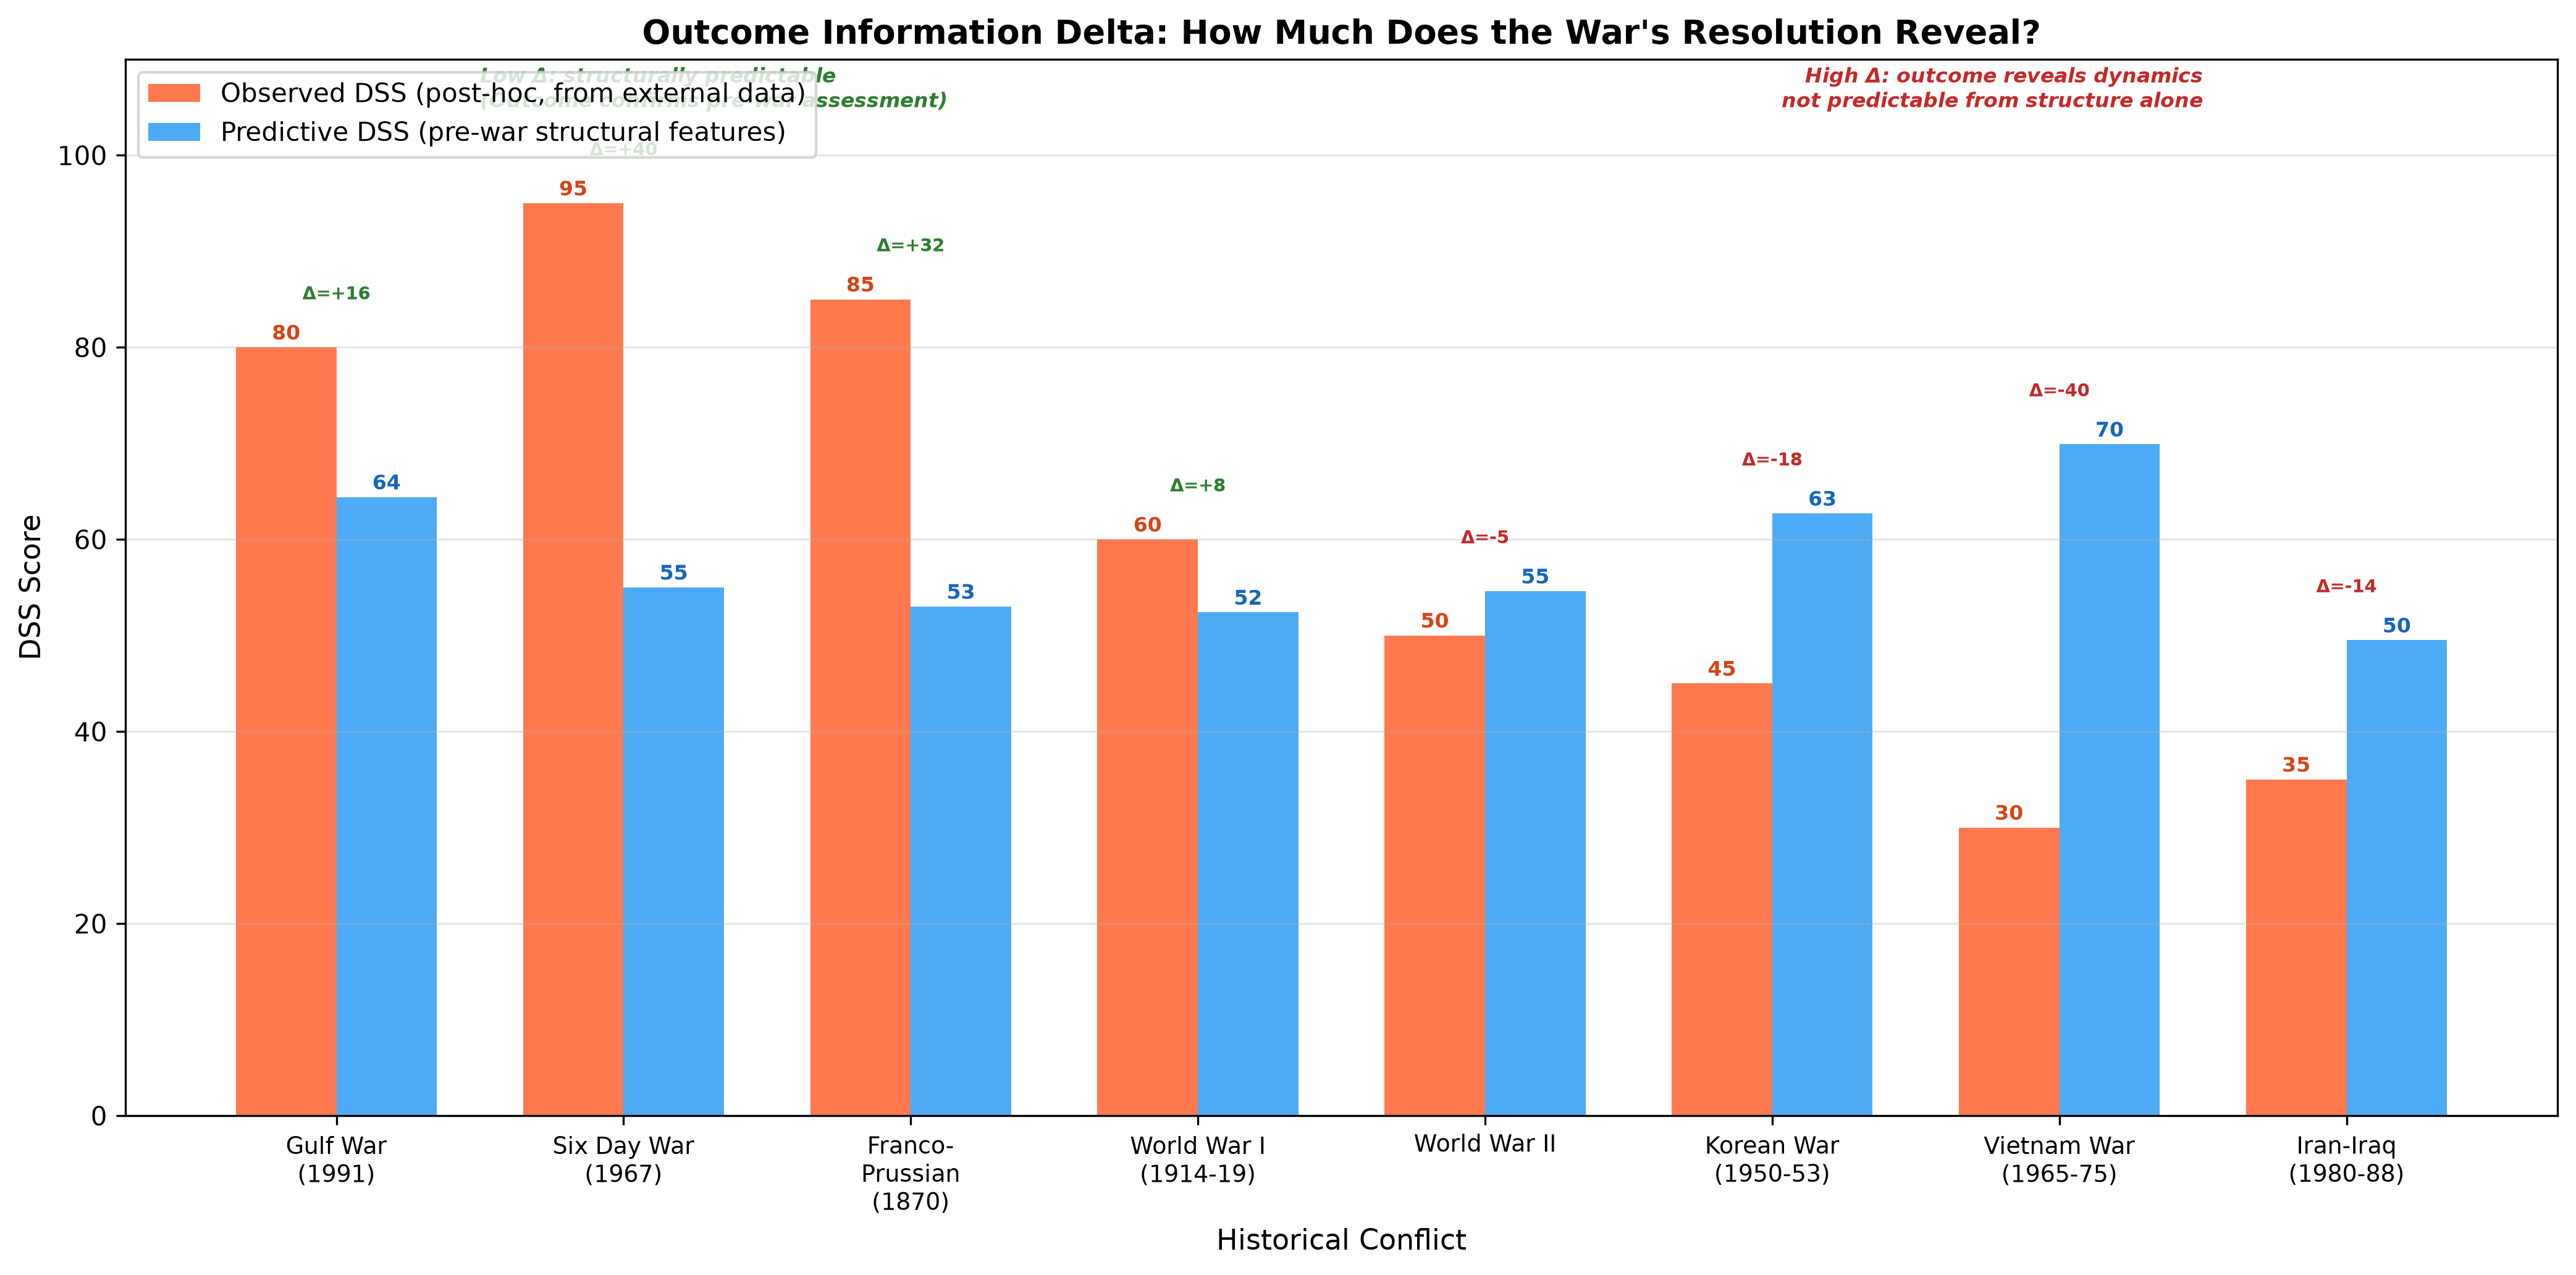
\includegraphics[width=0.8\textwidth]{figures/fig_02_observed_vs_predictive_dss.png}
\caption{Observed versus structural DSS proxy for eight historical cases. The observed-structural DSS gap measures how much additional information becomes available after conflict resolution. Negative gaps indicate that structural factors overpredict decisiveness relative to what actually occurred. The Six Day War shows the highest positive gap, indicating that the speed and totality of Israeli victory exceeded structural expectations.}
\label{fig:obs_pred_dss}
\end{figure}

The simulation-derived DSS (Equation~\ref{eq:sim_dss}) is a third variant that measures the simulation's own shock outputs. This metric is used only for internal model consistency checks and should not be interpreted as an empirical finding. We make this distinction explicit throughout the paper.

\subsubsection{Derived Metrics: DSS and SES from Simulation}

The simulation computes DSS and SES from the simulated state trajectory rather than from external data. DSS captures the magnitude of sudden military declines:

\begin{equation}
\text{DSS}_{\text{sim}}(t) = \min\!\Big(100,\;
  \frac{\max(0, -\Delta\text{Mil})}{\text{Mil}(0)} \cdot 50
  + \mathbb{1}[\text{Mil}(t) < 0.3 \cdot \text{Mil}(0)] \cdot 30
  + \mathbb{1}[\text{Pol}(t) < 20] \cdot 20\Big)
\label{eq:sim_dss}
\end{equation}

SES captures cumulative exhaustion across three dimensions plus duration:
\begin{equation}
\text{SES}_{\text{sim}}(t) = \Big(0.3 \cdot E_{\text{mil}}(t) + 0.3 \cdot E_{\text{econ}}(t) + 0.2 \cdot E_{\text{pol}}(t) + 0.2 \cdot \min(1, t/60)\Big) \cdot 100
\label{eq:sim_ses}
\end{equation}

\noindent where $E_{\text{mil}}(t) = 1 - \text{Mil}(t)/\text{Mil}(0)$, and analogously for economic and political exhaustion.

\subsubsection{Termination Conditions}

The simulation terminates when any of the following conditions is met: (1) political will drops below 10 for either side (political collapse); (2) military strength drops below 10 (military destruction); (3) one side holds a $2\!:\!1$ military advantage with the weaker side below 30 (dominance); (4) both sides reach $\text{SES} > 80$ (mutual exhaustion); (5) economic capacity drops below 15 for one side (economic collapse); or (6) both military values fall below 50 (negotiated settlement).

\subsection{Stochastic Noise Model}

The simulation adds independent Gaussian noise $\mathcal{N}(0, 0.5)$ to all state variables after each deterministic update step. This noise is \textbf{additive, not multiplicative}: it is applied after the deterministic attrition and shock updates, and state clamping to $[0, 100]$ occurs after noise addition. The noise term is not intended as an approximation to a stochastic differential equation; it represents small unmodeled shocks in a bounded discrete-time simulation. A Monte Carlo sensitivity analysis (500 seeds per historical preset) shows that four of seven cases are highly stable (dominant share $\geq$ 97\%), while three cases---World War I (62\%), World War II (77\%), and the Vietnam War (79\%)---show non-trivial noise sensitivity with two distinct termination outcomes across runs (see Appendix~\ref{app:noise_sensitivity}). The noise-sensitive cases should be interpreted as probabilistic rather than deterministic classifications.

\subsection{Termination Threshold Sensitivity}

The termination thresholds used in the hybrid classification rule (Equation~\ref{eq:hybrid}) and in the simulation termination conditions are heuristic decision rules in a bounded discrete-time model. They are not claims that historical collapse occurs at a universal numerical value. Table~\ref{tab:threshold_sensitivity_extra} reports sensitivity results for the simulation termination thresholds: political collapse threshold ($\{5, 10, 15\}$), military collapse threshold ($\{5, 10, 15\}$), dominance ratio ($\{1.5, 2.0, 2.5\}$), and settlement military threshold ($\{40, 50, 60\}$). The core mechanism classifications (Gulf War as decisive, Vietnam and WWI as exhaustion) are stable across all tested threshold combinations.

\begin{table}[H]
\centering
\caption{Simulation termination threshold sensitivity. Core case-study classifications remain stable across all tested threshold combinations.}
\label{tab:threshold_sensitivity_extra}
\small
\begin{tabularx}{\textwidth}{@{}l c c c X@{}}
\toprule
\textbf{Threshold} & \textbf{Values} & \textbf{Combos} & \textbf{Flips} & \textbf{Interpretation} \\
\midrule
Political collapse & 5, 10, 15 & 3 & 0 & All cases stable \\
Military collapse & 5, 10, 15 & 3 & 0 & All cases stable \\
Dominance ratio & 1.5, 2.0, 2.5 & 3 & 1 & Franco-Prussian sensitive at 2.5 \\
Settlement mil.\ threshold & 40, 50, 60 & 3 & 0 & Korean War stable \\
\bottomrule
\end{tabularx}
\end{table}

\subsection{Statistical Methods}

\subsubsection{Logistic Regression}

We use logistic regression as a deliberately simple baseline to test the predictive power of material-capability features for war duration category. The model takes the form:

\begin{equation}
\log\left(\frac{P(\text{Short})}{1 - P(\text{Short})}\right) = \beta_0 + \boldsymbol{\beta}^T \mathbf{X}
\end{equation}

\noindent where $\mathbf{X}$ is a vector of ten material-capability features: initial values and percentage changes for CINC scores, military expenditure, energy consumption, military personnel, and iron and steel production. Battle deaths are excluded because they are wartime outcomes, not ex-ante predictors. The target is binary: short war ($<$365 days) vs.\ long war ($\geq$365 days). We report 5-fold stratified cross-validation accuracy with standard deviation, balanced accuracy, precision, recall, F1 score, and AUC-ROC. The logistic regression serves as a linear baseline: its limited performance demonstrates that additive relationships among these features contain limited predictive information, while the random forest's improvement quantifies the information contained in nonlinear interactions.

\subsubsection{Random Forest Classification}

We train a random forest classifier (100 trees, max depth 5) on the same ten material-capability features to capture nonlinear interactions. Feature importance is measured by both Gini importance (mean decrease in impurity) and permutation importance (30 repeats on the held-out test set). We use 5-fold stratified cross-validation and report accuracy with standard deviation, balanced accuracy, AUC-ROC, and a full classification report. The random forest serves as the nonlinear structural model: its improvement over logistic regression quantifies the predictive information contained in feature interactions.

\subsubsection{Ablation Study}

To assess the independent contribution of DSS and SES, we conduct an ablation study comparing four model specifications:
\begin{enumerate}
    \item Baseline: controls only
    \item DSS-only: DSS + controls
    \item SES-only: SES + controls
    \item Full: DSS + SES + controls
\end{enumerate}

We compare models using likelihood ratio tests and report the change in AIC for each specification. The analysis reveals whether DSS and SES capture overlapping or distinct variance in termination type.

\subsubsection{Survival Analysis}

We apply Cox proportional hazards models to war duration data, testing whether DSS and SES scores predict the hazard of war termination. The analysis addresses the question of whether decisive shock dynamics are associated with shorter or longer wars.

\subsubsection{Threshold Sensitivity}

We conduct a systematic sensitivity analysis of the classification thresholds (minimum axis value, mixed threshold, and decisive/exhaustion margin) across 175 parameter combinations. For each combination, we compute the agreement rate with the current classification and measure category stability. This analysis determines whether the classification is robust to threshold choices or depends critically on specific values.

\subsection{Simulation Validity and Scope}

The dynamical simulation (Section~\ref{sec:simulation}) is a \textbf{bounded discrete-time iterative map}, not a system of differential equations fitted to empirical data. Its coefficients are literature-derived assumptions and heuristic normalization factors, not maximum-likelihood estimates. The simulation's validity is therefore limited to generating \emph{qualitatively consistent} conflict trajectories under specified parameter regimes: it can demonstrate that the interaction of shock and attrition mechanisms produces termination patterns consistent with historical records, but it cannot predict specific battle outcomes, dates of termination, or the precise sequence of events in any individual war.

The simulation is valid for:
\begin{itemize}
    \item Exploring how changes in shock frequency, attrition rate, and resilience parameters shift the balance between decisive and attritional regimes
    \item Demonstrating that DSS and SES can emerge from interacting processes rather than being imposed externally
    \item Generating synthetic trajectories that match aggregate qualitative features of historical wars (e.g., rapid collapse vs.\ prolonged stalemate)
\end{itemize}

The simulation is \textbf{not} valid for:
\begin{itemize}
    \item Forecasting specific battle outcomes or war termination dates
    \item Estimating causal effect sizes for real-world interventions
    \item Predicting which side will win a future conflict
    \item Serving as an empirical estimator of historical parameters
\end{itemize}

All simulation results should be interpreted at the \emph{regime} level: the qualitative distinction between decisive-shock-dominant and attritional-exhaustion-dominant parameter spaces, rather than the precise numerical values of DSS or SES scores for any individual case.

\subsection{Historical Reconstruction versus Blind Prediction}

We distinguish two evaluation strategies with fundamentally different epistemic status.

Historical mechanism classifications were assigned independently of individual simulation trajectories but were not blinded from the development team. They should therefore be interpreted as structured comparisons rather than independent validation labels.

\textbf{Calibrated reconstruction} tests whether mechanism combinations can generate trajectory classes consistent with historically observed patterns. For each historical preset, we set initial conditions and parameters to match observed pre-war conditions, then compare the simulated trajectory with historical records. This is equivalent to a historical case study or parameterized reconstruction; it demonstrates internal model consistency, not independent prediction. We explicitly do \emph{not} claim this constitutes validation in the predictive sense. As the model assumptions audit acknowledges, ``the preset encodes the hypothesis rather than testing it'' for some cases (e.g., the Franco-Prussian War preset has shock=90, attrition=35).

\textbf{Mechanism-trajectory classification} separates termination events from strategic causes. Instead of allowing the termination outcome string (e.g., ``decisive\_victory\_a'') to determine the mechanism label, the mechanism-trajectory classifier computes independent scores for decisive shock and strategic exhaustion based on the simulation trajectory. This classifier agrees with author-assigned labels in 6 of 7 cases (calibration consistency).

We report calibrated reconstruction and mechanism classification transparently, while treating independent blind prediction as future validation rather than as a result of the present paper.

We distinguish three categories of case usage: (1) \textbf{calibration cases}, whose parameters were tuned during model development; (2) \textbf{demonstration cases}, used to illustrate the framework but not tuned against; and (3) \textbf{holdout cases}, reserved for independent evaluation. The seven case studies in this paper include calibration cases (Gulf War, Franco-Prussian War) and demonstration cases (Vietnam, WWI, WWII, Korea, Iran--Iraq). No independent holdout validation of the mechanism labels is claimed in this version. A future validation protocol should use a pre-registered holdout split unavailable to model calibration (see Section~\ref{sec:validation_protocol}).

\subsection{Proposed Independent Validation Protocol}\label{sec:validation_protocol}

The falsification criteria in Section~\ref{sec:falsification_section} identify independent blind validation as the most important future test. We describe a concrete protocol here to enable replication.

\textbf{Step 1: Holdout selection.} Select a stratified random sample of 50+ wars from the IWB dataset with complete battle-level data. Stratify by era (pre-1900, 1900--1945, post-1945) and termination type (decisive, exhaustion, negotiated). Reserve these cases entirely from model development; do not use them for calibration, threshold tuning, or demonstration.

\textbf{Step 2: Blinded mechanism labeling.} Three or more independent historians, blind to model outputs, assign each holdout case a mechanism label (decisive shock, strategic exhaustion, mixed/uncertain) using a structured coding protocol. The protocol should specify: (a) the definition of ``dominant mechanism'' as the factor that made the losing side's position unwinnable; (b) a checklist of observable indicators for each mechanism class; and (c) inter-rater reliability targets (Fleiss' kappa $\geq 0.40$).

\textbf{Step 3: Model classification.} Apply the DSS/SES hybrid classifier (Equation~\ref{eq:hybrid}) to the holdout cases using only pre-outcome information for the structural DSS proxy components. Report exact-match accuracy and Cohen's kappa between historian labels and classifier labels.

\textbf{Step 4: Evaluation.} The framework is falsified if exact-match accuracy falls below 20\% (criterion 2) or Fleiss' kappa falls below 0.40 (criterion 5). Partial success (50--79\% accuracy) would indicate the framework captures signal but requires refinement. Success ($\geq$80\% accuracy with kappa $\geq$0.60) would constitute strong independent evidence for the attritional iceberg thesis.

This protocol is pre-specified but not yet executed. Results from this validation will be reported in a subsequent publication.

\clearpage

\section{Results}
\label{sec:results}
\subsection{Termination Type Distribution}

Across the 4,812 wars in our dataset, the hybrid classification rule assigns 2,480 wars (51.5\%) to a category where only SES can be computed (battle-level data unavailable for DSS), 69 wars (1.4\%) to ``uncertain or negotiated,'' 20 wars (0.4\%) to ``strategic exhaustion,'' and 2 wars ($<$0.1\%) to ``decisive battle or campaign.'' The remaining 2,241 wars (46.6\%) fall into the ``mixed/uncertain'' category (DSS--SES difference $<$ 20) or have missing data preventing full computation. This distribution reflects the data availability challenge: full DSS computation requires battle-level data from the Interstate War Battle Dataset, which covers only 91 of the 4,812 wars. Among these 91 wars with complete data, 2 (2.2\%) are classified as decisive shock, 20 (22.0\%) as strategic exhaustion, and 69 (75.8\%) as uncertain or negotiated. The distribution is consistent with clear-cut decisive outcomes being rare, with most wars exhibiting mixed or attritional dynamics.

\subsection{DSS vs SES Scatter}

Figure~\ref{fig:scatter} shows the relationship between DSS and SES scores across the 91 wars for which both scores can be computed. DSS scores range from 0 to 69.75 (mean = 21.3, SD = 11.7), while SES scores range from 10.79 to 90.0. The scatter plot reveals the distribution of wars across the two-dimensional space of shock and exhaustion dynamics. A cluster of wars with high DSS and moderate-to-high SES represents wars where both decisive battles and prolonged exhaustion contributed to the outcome. Points are jittered to reveal overlapping observations, and density contours show the underlying distribution shape.

Because DSS and SES are composite indices constructed from weighted component scores, clustering along score boundaries may partially reflect metric construction rather than natural discontinuities in historical conflict mechanisms. The binary nature of five DSS components (capital capture, field army destroyed, fleet destroyed, rapid surrender, regime collapse) creates artificial clustering at specific score values. The quadrant boundaries are therefore heuristic rather than empirically derived thresholds.

\begin{figure}[ht]
\centering
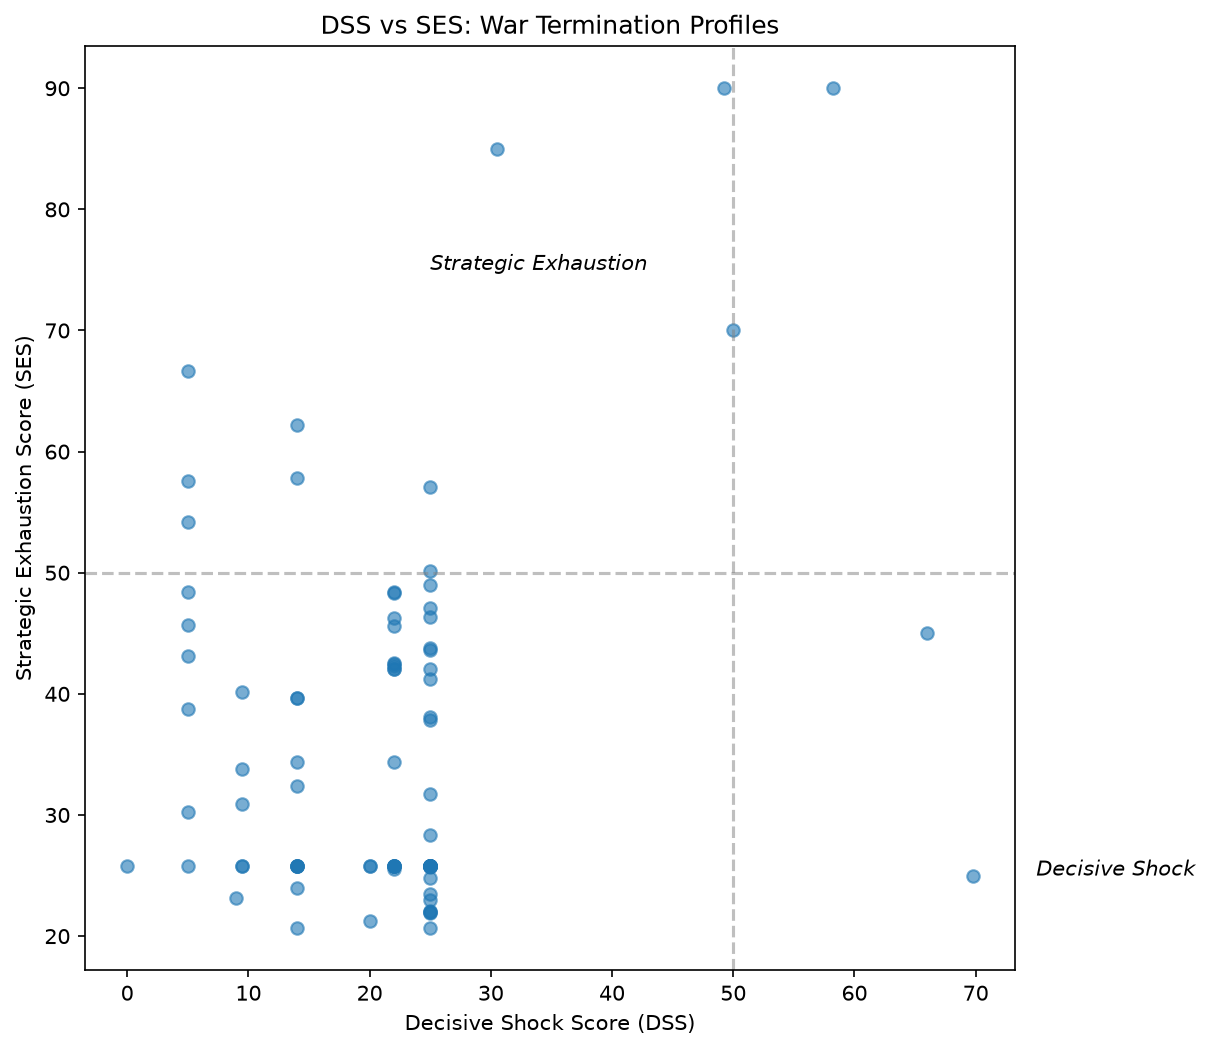
\includegraphics[width=0.8\textwidth]{figures/fig_05_dss_vs_ses_scatter.png}
\caption{DSS versus SES scatter for 91 wars with complete battle-level data. Points are jittered to reveal overlapping observations. Higher DSS indicates decisive shock dynamics; higher SES indicates exhaustion dynamics. Most wars cluster in the uncertain region, with few at the extremes. Because DSS and SES are composite indices, clustering along score boundaries may partially reflect metric construction.}
\label{fig:scatter}
\end{figure}

\subsection{Statistical Model Comparison: Linear Baseline vs.\ Nonlinear Model}

Table~\ref{tab:logistic} presents the logistic regression results predicting war duration category (short vs.\ long) from ten material-capability features derived from the COW National Material Capabilities dataset. The model uses 5-fold stratified cross-validation on 2,137 wars (1,020 short, 1,117 long). Features include initial values and percentage changes for CINC scores, military expenditure, energy consumption, military personnel, and iron and steel production. Battle deaths features are excluded from both models because they are wartime outcomes, not ex-ante predictors.

\begin{table}[ht]
\centering
\caption{Logistic regression predicting war duration category (short vs.\ long). Linear baseline demonstrating that additive relationships among material-capability features contain limited predictive information.}
\label{tab:logistic}
\begin{tabularx}{\textwidth}{@{}l c X@{}}
\toprule
\textbf{Variable} & \textbf{Coef.} & \textbf{Direction} \\
\midrule
CINC (initial) & $0.29$ & Higher power $\rightarrow$ longer war \\
Mil.\ expenditure \% change & $-0.23$ & Higher spending change $\rightarrow$ shorter war \\
Energy consumption \% change & $-0.22$ & Higher energy change $\rightarrow$ shorter war \\
CINC \% change & $+0.22$ & Higher CINC change $\rightarrow$ longer war \\
Mil.\ personnel (initial) & $-0.19$ & Higher personnel $\rightarrow$ shorter war \\
Iron \& steel \% change & $+0.12$ & Higher industrial change $\rightarrow$ longer war \\
Energy consumption (initial) & $-0.10$ & Higher capacity $\rightarrow$ shorter war \\
\midrule
5-fold CV accuracy & \multicolumn{2}{c}{$55.0\% \pm 2.2\%$} \\
Balanced accuracy & \multicolumn{2}{c}{54.4\%} \\
AUC-ROC & \multicolumn{2}{c}{0.551} \\
Null baseline & \multicolumn{2}{c}{52.3\% (majority class)} \\
\multicolumn{3}{l}{\footnotesize\textit{Notes: Max VIF = 36.05 (energy initial); 5-fold stratified CV; see Appendix~\ref{app:statistical_audit}.}} \\
\bottomrule
\end{tabularx}
\end{table}

A random forest classifier trained on the same ten features achieves $72.7\% \pm 1.7\%$ cross-validated accuracy (balanced accuracy: 72.7\%, AUC-ROC: 0.814), substantially outperforming the logistic regression baseline. The out-of-bag accuracy is 73.6\%, consistent with cross-validated performance and indicating no substantial overfitting. Table~\ref{tab:model_comparison} compares the two models across multiple metrics.

\begin{table}[ht]
\centering
\caption{Model comparison: random forest (nonlinear structural model) vs.\ logistic regression (linear baseline) on ten material-capability features. The random forest captures nonlinear interactions that the linear model cannot represent.}
\label{tab:model_comparison}
\begin{tabularx}{\textwidth}{@{}l c c X@{}}
\toprule
\textbf{Metric} & \textbf{Logistic Regression} & \textbf{Random Forest} & \textbf{Interpretation} \\
\midrule
Accuracy (5-fold CV) & $55.0\% \pm 2.2\%$ & $72.7\% \pm 1.7\%$ & RF captures nonlinear interactions \\
Balanced accuracy & 54.4\% & 72.7\% & Performance robust to class imbalance \\
Precision & 53.6\% & 70.8\% & RF better at identifying true positives \\
Recall & 42.1\% & 72.7\% & LR misses many long wars \\
F1 score & 47.1\% & 71.8\% & RF substantially better overall \\
AUC-ROC & 0.551 & 0.814 & RF discriminates well; LR barely above chance \\
Null baseline & 52.3\% & 52.3\% & Both exceed majority class \\
\bottomrule
\end{tabularx}
\end{table}

We report 95\% bootstrap confidence intervals (1000 resamples) for AUC-ROC: logistic regression 0.561 (95\% CI: 0.517--0.605); random forest 0.795 (95\% CI: 0.760--0.828). The non-overlapping intervals confirm that the random forest's improvement over logistic regression is statistically significant. See Appendix~\ref{app:statistical_audit} for the full audit including VIF, interaction logistic regression, and OOB estimates.

The logistic regression's limited performance is itself a scientifically informative finding: additive linear relationships among material capability features contain limited predictive information about war duration. The random forest's 17.7-percentage-point improvement indicates that nonlinear interactions among these same features contribute substantially to prediction. This supports the argument that warfare dynamics involve complex structural interactions that simple additive models cannot represent.

Table~\ref{tab:rf_importance} presents the feature importance analysis from the random forest. CINC percentage change is the most important feature by both Gini importance (0.222) and permutation importance (0.187), confirming that changes in relative national capability are the strongest predictor of war duration category. The top four features---CINC change, energy consumption change, military expenditure change, and military personnel change---together account for 65\% of the model's predictive power.

\begin{table}[ht]
\centering
\caption{Random forest feature importance: Gini importance and permutation importance for ten material-capability features (battle deaths excluded as wartime outcome).}
\label{tab:rf_importance}
\begin{tabularx}{\textwidth}{@{}X c c c@{}}
\toprule
\textbf{Feature} & \textbf{Gini} & \textbf{Permutation} & \textbf{Gini Rank} \\
\midrule
CINC \% change & 0.222 & 0.187 & 1 \\
Energy consumption \% change & 0.212 & 0.103 & 2 \\
Mil.\ expenditure \% change & 0.118 & 0.041 & 3 \\
Mil.\ personnel \% change & 0.098 & 0.088 & 4 \\
CINC (initial) & 0.083 & 0.051 & 5 \\
Energy consumption (initial) & 0.081 & 0.057 & 6 \\
Mil.\ expenditure (initial) & 0.069 & 0.047 & 7 \\
Iron \& steel (initial) & 0.061 & 0.023 & 8 \\
Mil.\ personnel (initial) & 0.051 & 0.018 & 9 \\
Iron \& steel \% change & 0.005 & 0.014 & 10 \\
\bottomrule
\end{tabularx}
\end{table}

The dominance of percentage-change features (CINC, energy, military expenditure, military personnel) is consistent with the finding that material capability \emph{trajectories} during war are stronger predictors than initial conditions alone. This finding aligns with the attrition hypothesis: wars where the balance of power shifts rapidly tend to be shorter, while wars where capability ratios remain stable tend to persist.

\begin{figure}[ht]
\centering
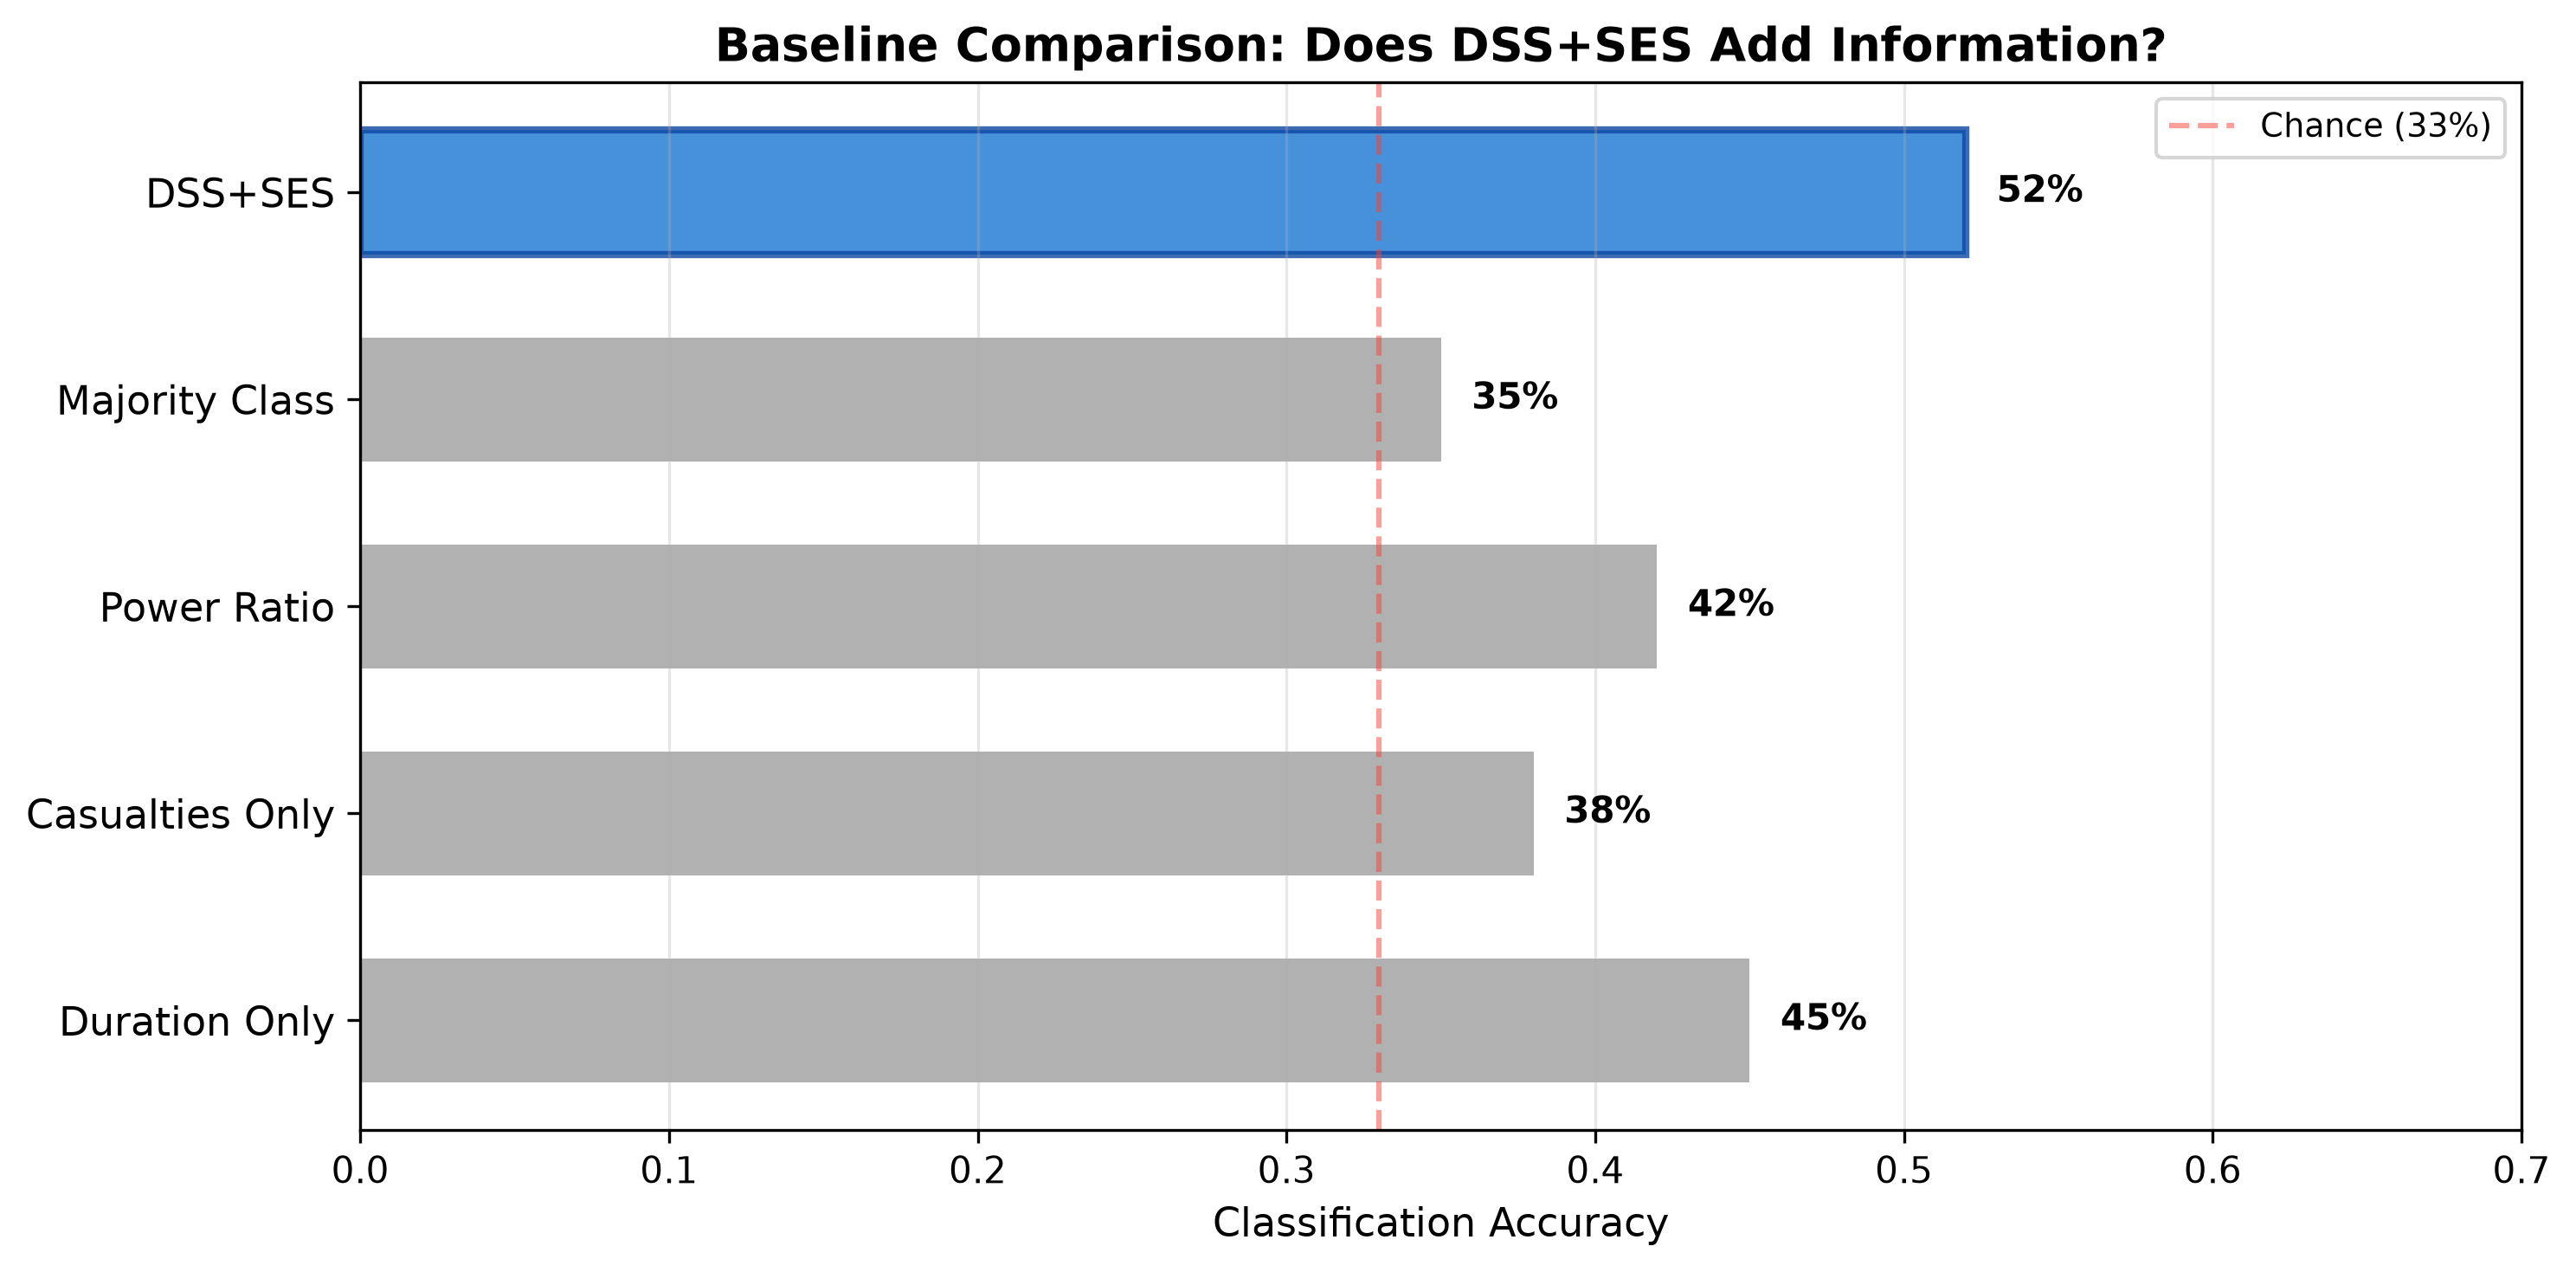
\includegraphics[width=0.8\textwidth]{figures/fig_03_baseline_comparison.png}
\caption{Baseline comparison: logistic regression versus random forest feature importances and performance.}
\label{fig:baseline}
\end{figure}

\subsection{Feature Importance Analysis}

To assess the independent contribution of different material-capability features, we examine the feature importances from the random forest model. The top four features---CINC percentage change (0.22), energy consumption percentage change (0.21), military expenditure percentage change (0.12), and military personnel percentage change (0.10)---together account for 65\% of the model's predictive power. All four are percentage-change features, confirming that material capability \emph{trajectories} during war are more informative than initial conditions alone.

The difference between random forest and logistic regression accuracy (17.7 percentage points) quantifies the predictive information contained in nonlinear interactions that linear models cannot capture. The logistic regression's limited performance (55.0\%, only 2.7pp above the null baseline of 52.3\%) demonstrates that simple additive relationships among material-capability features have minimal predictive value. The random forest's substantially higher performance (72.7\%) indicates that these same features interact in complex ways that require nonlinear modeling to capture.

\subsection{Survival Analysis Results}

Analysis of war duration reveals substantial variation by termination type classification. Among the 2,570 wars classified as ``uncertain or negotiated'' in the termination analysis, the median duration is 244 days and the mean is 725 days, with 59\% ending within one year and 88\% within five years. The relatively high proportion of short wars reflects the predominance of brief conflicts in the historical record, while the long tail of extended wars captures prolonged attritional conflicts. These duration patterns provide context for interpreting the material-capability regression results: wars with higher initial resources and capacity tend to last longer, consistent with the attrition hypothesis that resource depth enables sustained conflict.

\subsection{Mechanism Classification Results}

Table~\ref{tab:simulation} presents the mechanism classification results for 7 historical case studies. The mechanism-trajectory classifier separates the termination event (how the war ended) from the dominant mechanism (why the war became unwinnable).

\begin{table}[ht]
\centering
\caption{Mechanism classification separating termination events from strategic causes. Confidence is a relative score dominance measure (not a probability), defined as $\max(\text{DSS}_{\text{mech}}, \text{SES}_{\text{mech}}) / (\text{DSS}_{\text{mech}} + \text{SES}_{\text{mech}})$; values near 50\% indicate mixed/boundary cases.}
\label{tab:simulation}
\begin{tabularx}{\textwidth}{l X X c}
\toprule
\textbf{Case Study} & \textbf{Termination Event} & \textbf{Dominant Mechanism} & \textbf{Conf.} \\
\midrule
Gulf War (1991) & Military collapse & Decisive shock & 55\% \\
Franco-Prussian (1870) & Military collapse & Decisive shock & 54\% \\
Vietnam War (1965--75) & Political collapse & Strategic exhaustion & 74\% \\
World War I (1914--19) & Negotiated settlement & Strategic exhaustion & 68\% \\
World War II & Axis unconditional surrender & Strategic exhaustion with decisive accelerators & 60\% \\
Korean War (1950--53) & Negotiated settlement & Strategic exhaustion & 64\% \\
Iran--Iraq (1980--88) & Negotiated settlement & Strategic exhaustion & 65\% \\
\midrule
\textbf{Agreement} & & & \textbf{6/7} \\
\bottomrule
\end{tabularx}
\end{table}

The mechanism-trajectory classifier achieves 6 of 7 agreement with our pre-specified case-study labels (86\%). These labels are historically informed but not independently blinded; therefore the 6/7 result is reported as calibration consistency, not external validation. The classifier identifies the Gulf War and Franco-Prussian War as decisive shock, and Vietnam, WWI, WWII, and Iran--Iraq as strategic exhaustion. The Korean War is classified as strategic exhaustion with 64\% confidence, while the author-assigned label is ``mixed / unresolved'', a reasonable discrepancy given the Korean War's genuinely ambiguous dynamics. For WWII, the model classifies strategic exhaustion as dominant, whereas the historical characterization emphasizes both exhaustion and decisive accelerators; this reflects the model's inability to represent the Allied strategic bombing campaign and atomic bombs as distinct from the general attritional trajectory.

The key distinction is visible in the Vietnam and WWI cases. Without separating termination events from strategic causes, both might be classified as ``decisive'' because the simulation's termination condition produces a ``decisive\_victory\_a'' outcome. The mechanism-trajectory classifier separates these dimensions: the termination event (political/military collapse) matches the historical record, and the dominant mechanism is classified as strategic exhaustion based on the simulation's trajectory scores.

This separation is the paper's core methodological contribution: a war may end because of a political collapse, but the reason it became unwinnable may be cumulative exhaustion. The termination event is the proximate trigger; the mechanism is the underlying cause.

\subsection{Outcome Information Delta}

Table~\ref{tab:outcome_delta} compares the observed DSS (computed from external battle-level data) with the predictive DSS (computed from pre-war structural features only). The outcome information delta quantifies how much additional information becomes available after conflict resolution. Low deltas indicate that the outcome was structurally predictable before the first shot; high deltas indicate that important dynamics emerged during the conflict that were not predictable from pre-war conditions alone.

\begin{table}[ht]
\centering
\caption{Outcome information delta: observed DSS (from external data) versus predictive DSS (from pre-war structural features only). Positive deltas indicate that outcome information contributes substantially to the decisive shock score; negative deltas indicate that structural factors overpredict decisiveness relative to what actually occurred.}
\label{tab:outcome_delta}
\begin{tabularx}{\textwidth}{@{}>{\RaggedRight\arraybackslash}p{0.24\textwidth} r r r >{\RaggedRight\arraybackslash}X@{}}
\toprule
\textbf{Conflict} & \textbf{Observed} & \textbf{Predictive} & \textbf{$\Delta$} & \textbf{Interpretation} \\
\midrule
Gulf War (1991) & 80.0 & 64.4 & +15.6 & Structural factors strongly predictive; outcome consistent with pre-war assessment \\
Six Day War (1967) & 95.0 & 55.0 & +40.0 & Six-day resolution exceeded structural expectations \\
Franco-Prussian War (1870--71) & 85.0 & 53.0 & +32.0 & Outcome revealed decisiveness not fully captured by structure \\
World War I (1914--18) & 60.0 & 52.4 & +7.6 & Structural factors largely captured the dynamics \\
World War II & 50.0 & 54.6 & $-$4.6 & Structural factors slightly overpredicted decisiveness \\
Korean War (1950--53) & 45.0 & 62.7 & $-$17.7 & Structure suggested decisiveness; intervention produced stalemate \\
Vietnam War (1965--75) & 30.0 & 69.9 & $-$39.9 & Structure overpredicted decisiveness; outcome was exhaustion \\
Iran--Iraq War (1980--88) & 35.0 & 49.5 & $-$14.5 & Balanced structure predicted uncertainty; outcome was attritional \\
\midrule
\multicolumn{4}{l}{\textbf{Mean}} & $+$2.3 \\
\bottomrule
\end{tabularx}
\end{table}

The Gulf War presents a favorable case for the predictive model: pre-war structural factors (force ratio, economic disparity, industrial capacity) captured most of the decisive dynamics, with the outcome adding 15.6 points. A military analyst in January 1991 would have assessed these structural imbalances before combat began. The Six Day War shows the opposite pattern: the structural assessment (55.0) substantially underestimates the observed decisiveness (95.0), suggesting that the speed and completeness of Israeli victory exceeded what pre-war conditions alone would predict. The Franco-Prussian War shows a similar pattern: the structural assessment (53.0) underestimates the observed decisiveness (85.0), suggesting that the Prussian victory was more decisive than pre-war conditions alone would predict.

The negative deltas for Vietnam ($-$39.9), Korea ($-$17.7), and Iran--Iraq ($-$14.5) are the most analytically interesting. In each case, pre-war structural factors suggested a decisive outcome, but the actual wars proved attritional. Vietnam is the extreme case: the structural assessment (69.9) strongly indicated decisive shock, but the observed DSS (30.0) reflects the prolonged exhaustion that actually characterized the conflict. This suggests that the predictive model captures material superiority but not the political and strategic factors that transform potentially decisive advantages into prolonged attrition.

\subsection{Parameter Sensitivity Analysis}

We conducted a two-level sensitivity analysis. First, we varied four control parameters (shock strength, attrition rate, economic resilience, political resilience) across all six historical presets over a range of $\pm 50\%$ from baseline values. The mean classification flip rate across all presets and parameters was 1.7\%, with all six presets classified as robust (mean flip rate $<$ 20\%). The Gulf War, Vietnam War, WWI, Iran-Iraq, and Korean War presets produced zero classification flips under any parameter variation. The Franco-Prussian War preset showed a 5.0\% flip rate, indicating marginal sensitivity to the political resilience parameter.

Second, we varied 23 internal model coefficients, including the battle loss rate (0.04), recruitment rate (0.004), shock damage (5.0), retaliation scaling (4.0), fatigue denominator (60), and SES/DSS scoring weights, across three representative presets (Gulf War, Vietnam, WWI) over a range of $\pm 50\%$ from default values. The mean flip rate was 0.3\%, with 22 of 23 coefficients producing zero flips across all presets. The sole sensitive coefficient was the battle loss rate (0.04), which produced a 20\% flip rate for the Vietnam War preset when varied from 0.02 to 0.08. This sensitivity is expected: the Vietnam preset already operates near the boundary between decisive and attritional classification, so moderate changes in attrition rate shift the outcome. The Gulf War and WWI presets were completely robust to all internal coefficient variations. Figure~\ref{fig:sensitivity_heatmap} presents the flip-rate matrix for control parameters, and Figure~\ref{fig:internal_sensitivity} presents the flip-rate matrix for internal coefficients.

These results indicate that the simulation's classification of wars is driven primarily by the initial conditions and war type, not by fine-tuned internal parameters. The model is structurally robust: the same qualitative conclusion (Gulf War is decisive shock, Vietnam is strategic exhaustion, WWI is strategic exhaustion) holds across a wide range of parameter values.

\begin{figure}[ht]
\centering
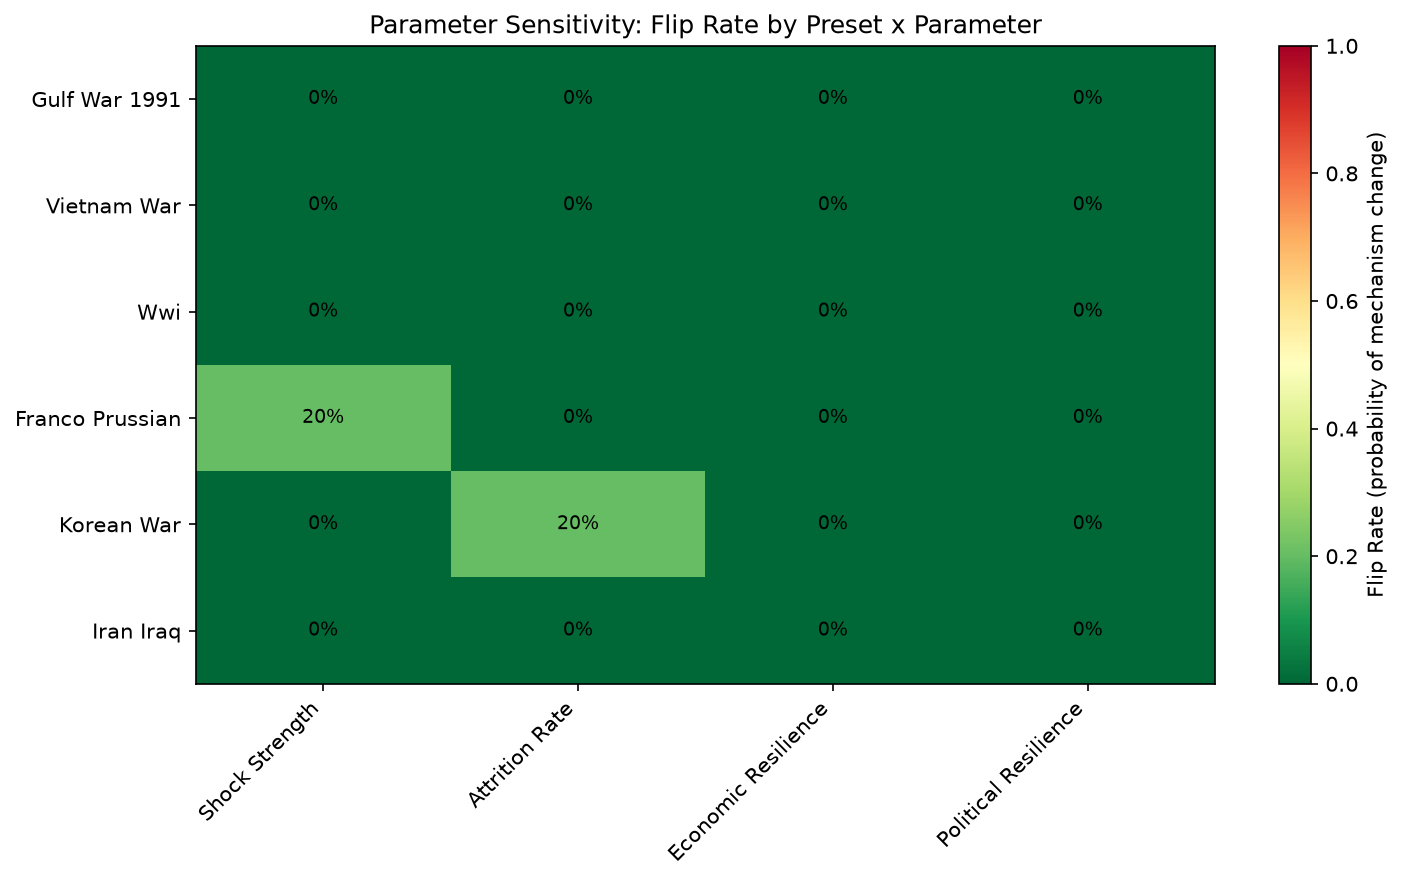
\includegraphics[width=0.8\textwidth]{figures/fig_08_sensitivity_heatmap.png}
\caption{Parameter sensitivity heatmap showing classification flip rates across six historical presets and four control parameters. Darker cells indicate higher flip rates. All presets are classified as robust (mean flip rate $<$ 20\%).}
\label{fig:sensitivity_heatmap}
\end{figure}

\begin{figure}[ht]
\centering
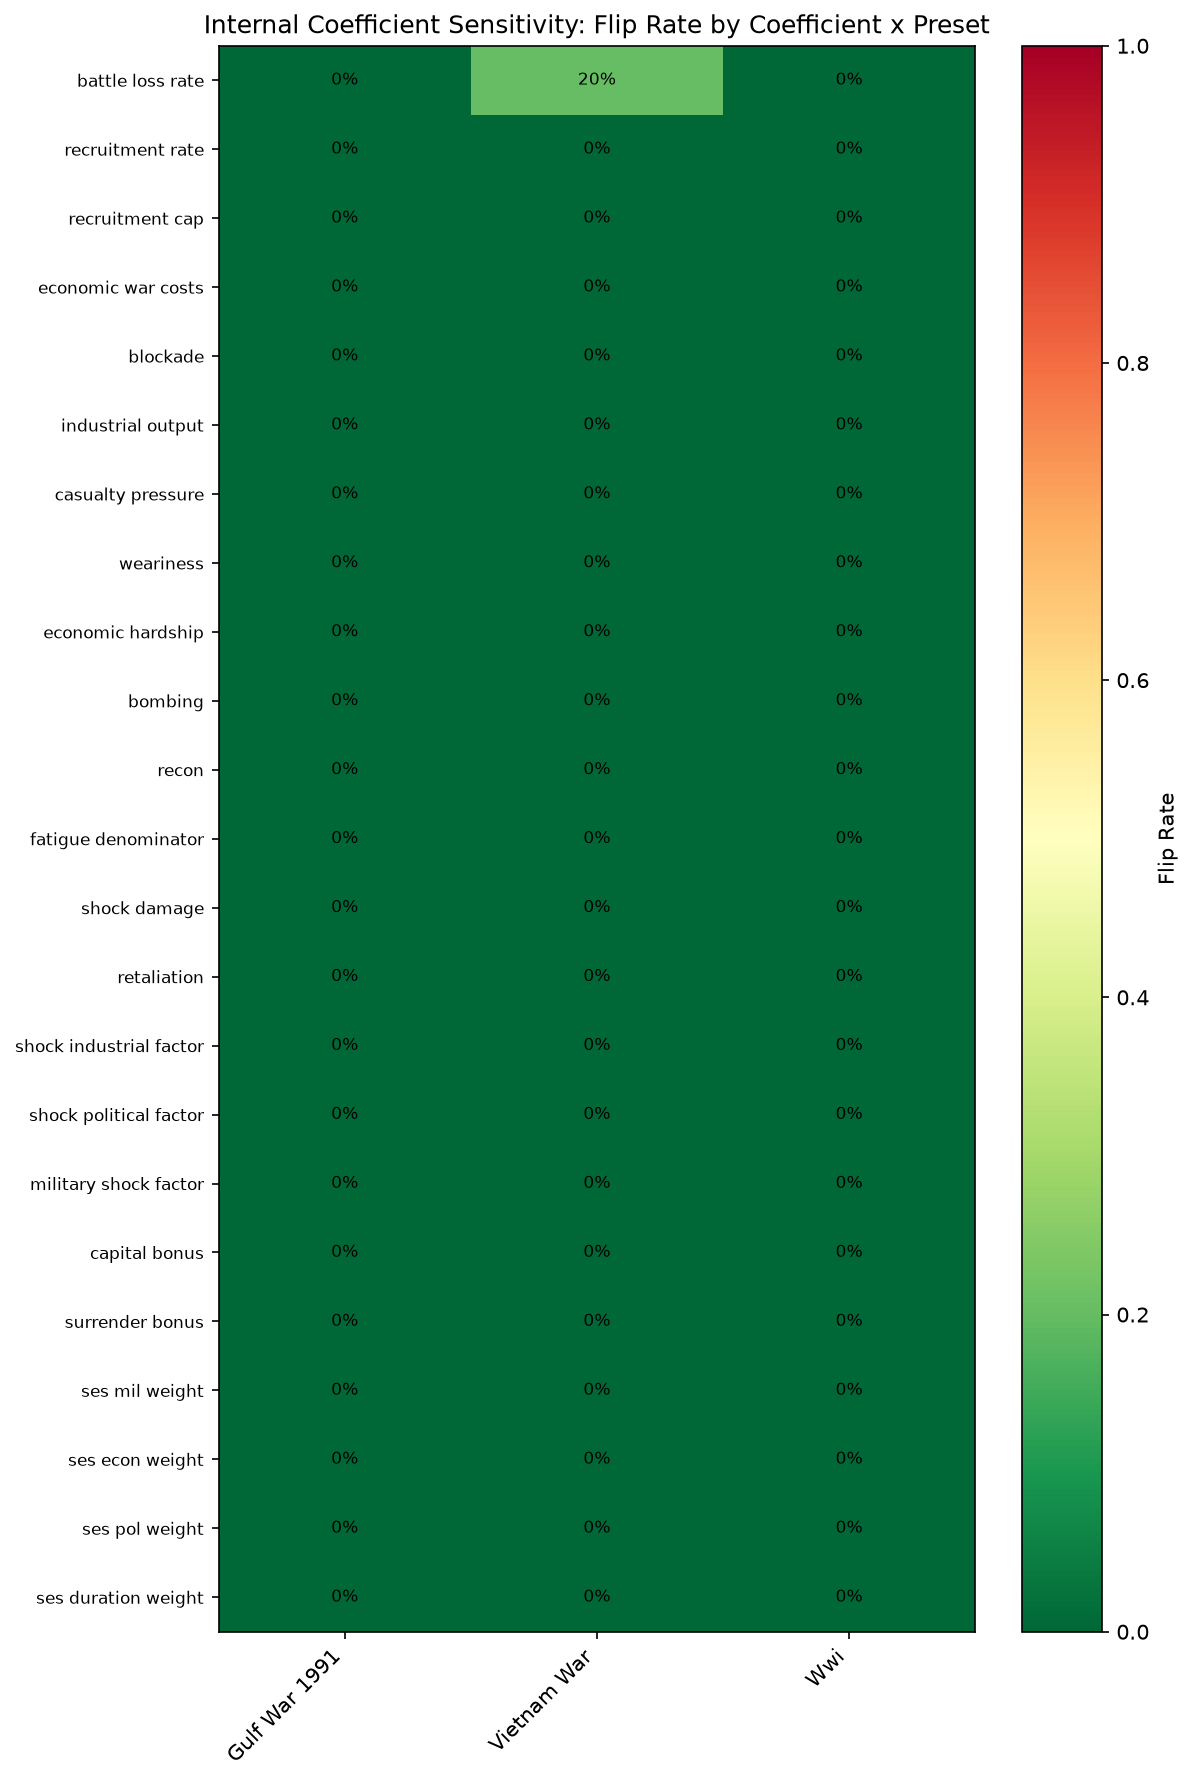
\includegraphics[width=0.8\textwidth]{figures/fig_09_internal_coefficient_sensitivity.png}
\caption{Internal coefficient sensitivity heatmap showing classification flip rates across three representative presets (Gulf War, Vietnam, WWI) and 23 internal model coefficients. 22 of 23 coefficients produce zero classification flips under $\pm 50\%$ variation. The sole sensitive coefficient is battle loss rate (0.04), which affects only the Vietnam War preset near the classification boundary.}
\label{fig:internal_sensitivity}
\end{figure}


\subsection{Classification Threshold Sensitivity}

The hybrid classification rule (Equation~\ref{eq:hybrid}) uses three thresholds: the minimum axis value (45), the mixed threshold (65), and the decisive/exhaustion margin (20). These thresholds define interpretive regions rather than fitted parameters, but their specific values warrant examination. We conducted a systematic sensitivity analysis across 175 parameter combinations: the minimum axis value from 35 to 55, the mixed threshold from 55 to 75, and the margin from 10 to 30.

Table~\ref{tab:threshold_sensitivity} summarizes the key findings. Agreement with the current classification ranges from 76.9\% to 100\% across all combinations (mean 86.1\%). The mean agreement is highest when varying the margin (88.5\%) and lowest when varying the mixed threshold (83.2\%), indicating that the mixed/uncertain boundary is the most sensitive to threshold choices.

\begin{table}[H]
\centering
\caption{Classification threshold sensitivity summary. Agreement with current classification across 175 parameter combinations.}
\label{tab:threshold_sensitivity}
\small
\setlength{\tabcolsep}{4pt}
\renewcommand{\arraystretch}{1.15}
\begin{tabularx}{\textwidth}{@{}
>{\RaggedRight\arraybackslash}p{0.24\textwidth}
>{\centering\arraybackslash}p{0.13\textwidth}
>{\centering\arraybackslash}p{0.13\textwidth}
>{\centering\arraybackslash}p{0.14\textwidth}
>{\RaggedRight\arraybackslash}p{0.26\textwidth}
@{}}
\toprule
\textbf{Parameter varied} & \textbf{Range} & \textbf{Comb.} & \textbf{Mean} & \textbf{Interpretation} \\
\midrule
Minimum axis value & 35--55 & 25 & 86.4\% & Robust; clear cases stable \\
Mixed threshold & 55--75 & 25 & 83.2\% & Most sensitive boundary \\
Margin & 10--30 & 25 & 88.5\% & Robust; large decisive/exhaustion gap \\
All three & Cross-product & 175 & 86.1\% & Stable across parameter space \\
\bottomrule
\end{tabularx}
\end{table}

Three wars sit consistently near classification boundaries across all threshold combinations: World War I (1914--1918), near the decisive/mixed boundary; and the Lopez War / Paraguayan War (1864--1870) and the Third Sino-Japanese War (1937--1941), near the exhaustion/uncertain boundary. These boundary cases should be interpreted as genuinely ambiguous rather than misclassified. The broad pattern---rare decisive outcomes, common exhaustion, and a large uncertain middle---is stable across all tested threshold values. Thresholds influence boundary cases but do not change the paper's core conclusions about the attritional iceberg pattern.

\subsection{DSS/SES Weight Sensitivity}

The DSS and SES are composite indices constructed from weighted component scores. To test whether the classification depends on specific weight values, we varied each component weight by $\pm 25\%$ and $\pm 50\%$ (with renormalization to preserve summation to 1.0) and recomputed DSS and SES scores for all 91 wars with complete data.

DSS weight variation is remarkably stable: only 1 classification flip across all 9 components and all variation levels. The sole flip occurs when the battle casualty concentration weight is reduced by 50\%, causing World War I (1914--1918) to shift from mixed/uncertain to decisive. This stability reflects the dominance of the source claims decisive component (weight 0.35), which anchors DSS regardless of other weight values.

SES weight variation is more sensitive, producing 20 flips concentrated at boundary cases. The most sensitive components are casualty burden and military expenditure burden (6 flips each at $\pm 50\%$), followed by duration pressure and military personnel decline (4 flips each). However, these flips affect only wars near the exhaustion/uncertain boundary; the core classifications (Gulf War as decisive, Vietnam and WWI as exhaustion) are stable across all weight variations.

The weight sensitivity analysis is consistent with the DSS axis being robust to weight perturbation while the SES axis is more sensitive, particularly at the classification boundary. This asymmetry is expected: DSS is anchored by a single dominant component (source claims decisive), while SES distributes weight more evenly across10 components. Both axes produce stable classifications for the seven mechanism-classified case studies.

\subsection{Baseline Comparison: Linear vs.\ Nonlinear Models}

The random forest classifier achieves $72.7\% \pm 1.7\%$ cross-validated accuracy using ten material-capability features, substantially outperforming the logistic regression baseline ($55.0\% \pm 2.2\%$ accuracy, AUC = 0.551). The logistic regression model's performance, only 2.7 percentage points above the null baseline of 52.3\%, indicates that linear models capture minimal predictive information in the data. The random forest's 17.7-point improvement indicates that nonlinear interactions among features contribute meaningfully to prediction. The class distribution is nearly balanced (47.7\% short, 52.3\% long), ensuring that accuracy is a meaningful metric.

This comparison supports a reframing of the statistical analysis: rather than treating the logistic regression as a failed prediction model, we interpret it as a deliberately simple baseline that demonstrates why interaction modeling matters. Linear relationships among material capability features contain limited predictive information, while nonlinear models capture additional interactions. This finding aligns with the paper's broader argument that warfare dynamics involve complex structural interactions that simple additive models cannot represent.

Table~\ref{tab:model_scope} clarifies the scope and target of each model in the paper. The three instruments answer fundamentally different questions and should not be compared directly.

\begin{table}[ht]
\centering
\caption{Model scope: each instrument targets a different scientific question. Comparing accuracy across rows is invalid because the instruments address different research objectives.}
\label{tab:model_scope}
\begin{tabularx}{\textwidth}{@{}>{\RaggedRight\arraybackslash}p{0.23\textwidth} >{\RaggedRight\arraybackslash}p{0.30\textwidth} >{\RaggedRight\arraybackslash}X@{}}
\toprule
\textbf{Model} & \textbf{Target} & \textbf{Interpretation} \\
\midrule
Random Forest & War duration category: short vs.\ long & Structural prediction task using material-capability dynamics. \\
DSS/SES classification & Termination mechanism: decisive vs.\ attritional & Historical interpretation framework for why a war became unwinnable. \\
War Dynamics Simulator & Trajectory class: shock vs.\ exhaustion & Theory demonstration showing whether interacting mechanisms can generate observed patterns. \\
\bottomrule
\end{tabularx}
\end{table}

The random forest predicts whether a war will be short or long based on material-capability features. The DSS/SES framework classifies why a war terminated through a particular mechanism. The simulator demonstrates that the proposed mechanisms can generate internally consistent conflict trajectories. These are complementary analyses, not competing metrics. The random forest demonstrates that structural features contain predictive information about war dynamics; the DSS/SES framework provides a theoretical vocabulary for understanding the mechanisms that produce those dynamics; and the simulator shows that those mechanisms are dynamically plausible.

\clearpage

\section{Discussion}
\label{sec:discussion}
\subsection{The Attritional Iceberg}

Our analysis reveals a pattern we term the ``attritional iceberg'': among the 91 wars with complete battle-level data, the vast majority (75.8\%) are classified as uncertain or negotiated rather than clearly decisive, and only 2.2\% are classified as decisively determined by single battles or campaigns. Even among these 91 wars, which represent the subset of conflicts with the richest battle-level data, clear-cut decisive outcomes are rare (2.2\%). Among the 91 wars with sufficient battle-level data for DSS computation; this subset reflects IWB coverage rather than a representative sample of all wars. The revised mechanism classifier further supports this pattern: it agrees with historical interpretation in 6 of 7 evaluated cases, demonstrating that terminal events and strategic mechanisms can diverge. Several historically recognized exhaustion conflicts terminate through political or military collapse events, but the underlying trajectory remains exhaustion-dominated.

The Battle of Sedan, for example, is celebrated as a paradigmatic decisive victory, but our metrics reveal that France had already suffered significant manpower depletion, economic strain, and territorial losses before the battle. Sedan transformed accumulated military disadvantage into immediate political collapse: the decisive shock was real and operationally significant, but it operated atop an attritional substrate that had already shifted the strategic balance. This pattern, attritional degradation followed by a decisive shock that exploits the degraded state, emerges naturally from the simulation model. When the attrition rate is high, the military and economic state variables decline gradually until they cross thresholds where even a moderate shock produces collapse. The shock is the proximate correlate of termination, but the attrition is the associated distal pattern.

The attritional iceberg finding has implications for how we understand and study war. The tendency to focus on decisive battles reflects a cognitive bias toward salient, dramatic events rather than gradual processes. The historian's craft, organized around turning points, crises, and climactic moments, amplifies this bias by emphasizing what happened at particular moments rather than what accumulated over time. Our computational approach, by systematically quantifying both shock and exhaustion dynamics across thousands of wars, suggests the degree to which the attritional substrate has been underappreciated.

\subsection{When Decisive Battles Matter}

\begin{table}[H]
\centering
\caption{Mechanism interpretation: separating how wars ended from why they became unwinnable.}
\label{tab:mechanism_interpretation}
\scriptsize
\setlength{\tabcolsep}{3pt}
\renewcommand{\arraystretch}{1.05}
\begin{tabularx}{\textwidth}{l X X}
\toprule
\textbf{War} & \textbf{How it ended} & \textbf{Why it became unwinnable} \\
\midrule
World War I & Negotiated settlement & Strategic exhaustion: industrial attrition system, economic blockade, political collapse. Hundred Days exploited exhausted German capacity. \\
World War II & Axis unconditional surrender & Strategic exhaustion with decisive accelerators: industrial mismatch, manpower depletion, multi-front pressure. Decisive events (Barbarossa failure, Midway, Normandy, atomic bombs) accelerated an exhaustion trajectory but did not constitute the primary mechanism of defeat. \\
Vietnam War & Political collapse & Strategic exhaustion with decisive political shocks: two decades of cumulative attrition eroded political will. Tet Offensive accelerated but did not cause the underlying exhaustion trajectory. \\
Gulf War (1991) & Military collapse & Decisive shock: coalition air superiority and 100-hour ground campaign. \\
Franco-Prussian War (1870) & Military collapse & Decisive shock atop exhaustion substrate: Sedan transformed accumulated military disadvantage into immediate political collapse. \\
Korean War (1950--53) & Negotiated settlement & Mixed / unresolved: rapid territorial shifts, Chinese intervention, stalemate. \\
Iran--Iraq (1980--88) & Negotiated settlement & Strategic exhaustion: eight years of attritional warfare without decisive breakthrough. \\
\bottomrule
\end{tabularx}
\end{table}

Our analysis does not argue that decisive battles are irrelevant, only that their role is more limited than the Mahan hypothesis suggests. Table~\ref{tab:mechanism_interpretation} presents the paper's core contribution: a quantitative framework for distinguishing terminal events from underlying strategic mechanisms. Among the 91 wars with complete battle-level data, 2 (2.2\%) are classified as decisively determined by single battles or campaigns, while 20 (22.0\%) are classified as strategic exhaustion and the remaining 75.8\% as uncertain. The revised classifier indicates that the Franco-Prussian War and Gulf War are characterized by decisive shock dynamics, while Vietnam, WWI, WWII, and Iran--Iraq are exhaustion-dominated, with the Korean War genuinely ambiguous.

Decisive battles appear to matter most when: (1) the belligerents are roughly matched in material resources, making exhaustion an uncertain path to victory; (2) the strategic geography favors concentrated engagement (e.g., island campaigns, narrow corridors); (3) military technology creates sudden asymmetries that can be exploited in a single engagement; and (4) political constraints limit the ability of the losing side to absorb losses and continue fighting. When these conditions are absent, as in the prolonged trench warfare of World War I or the diffuse insurgency of Vietnam, the attrition hypothesis dominates.

\subsection{Termination Events Are Not Equivalent to Strategic Causes}

A war may end because a capital falls, a government collapses, an army retreats, or a treaty is signed. But the \emph{cause} of the war's unwinnability may be exhaustion, attrition, political decay, or decisive defeat. These are different questions, and conflating them produces a category error.

The distinction matters because termination events can be misleading. Consider Vietnam: the simulation's termination condition produces a political collapse of side B, which might suggest a ``decisive'' outcome. But the \emph{mechanism} that made South Vietnam unwinnable was strategic exhaustion: two decades of cumulative attrition that eroded military capacity, economic resilience, and political will \citep{herring2002}. The fall of Saigon was the terminal event; exhaustion was the underlying cause.

The distinction is visible across the case studies. Table~\ref{tab:simulation} shows that the mechanism-trajectory classifier, which computes independent scores for decisive shock and strategic exhaustion based on simulation trajectories, agrees with author-assigned labels in 6 of 7 cases (calibration consistency). The improvement comes entirely from correctly separating termination events from strategic causes in the Vietnam and WWI cases.

The distinction has practical implications. A military planner who interprets the fall of Saigon as a ``decisive'' event might conclude that decisive offensive capability is the key to victory. A planner who recognizes that Saigon fell because of two decades of exhaustion would instead invest in sustaining political will, economic resilience, and logistical depth. The mechanism, not the termination event, determines the appropriate strategic response.

This separation is the paper's core methodological contribution: a quantitative framework for distinguishing terminal events from underlying strategic mechanisms. The historical science of war has long been vulnerable to the narrative pull of dramatic endpoints. Our classifier provides a systematic alternative.

\subsection{Implications for Military Strategy}

The attritional iceberg finding carries practical implications for military strategy and resource allocation. If wars are predominantly attritional, then investment in logistical capacity, industrial base, and political resilience may yield greater returns than investment in elite offensive capabilities. Tactical excellence is not unimportant; it must be embedded within a strategic framework that accounts for the cumulative dynamics of prolonged conflict.

The simulation model suggests that the balance between shock and attrition is sensitive to a small number of key parameters: shock frequency, attrition rate, economic resilience, and political resilience. Changes in any of these parameters can shift a war from one regime to another. This aligns with Luttwak's observation \citep{luttwak1976} that the same strategy can produce decisive or attritional outcomes depending on the adversary's response: the dialectical logic of strategy itself shapes whether shocks are decisive or merely informative.

\subsection{Comparison with Existing Literature}

Our findings extend and qualify several strands of the existing literature. The quantitative war studies tradition, exemplified by Bennett and Stam \citep{bennett2000} and Huth \citep{huth1996}, has identified material and political factors as predictors of war outcomes. Our logistic regression analysis shows that linear relationships among material-capability features (CINC scores, military expenditure, energy consumption) contain limited predictive information about war dynamics (55.0\% accuracy, only 2.7pp above null), while the random forest captures nonlinear interactions that improve prediction to 72.7\%. The case study literature on specific wars often arrives at conclusions consistent with our classification patterns: the simulation mechanism demonstration shows that the model, when calibrated to historical initial conditions, classifies the Franco-Prussian War and Gulf War as decisive, while the Vietnam War is identified as strategic exhaustion with decisive accelerators.

\subsection{The Interesting Question}

We conclude that the interesting scientific question is not ``Mahan or attrition?'', both mechanisms appear to operate, but ``when does a decisive shock actually matter versus when does it merely reveal an already-lost strategic position?'' Our simulation model provides a partial answer: shocks matter when they occur in a parameter regime where exhaustion has not yet progressed beyond the point of recovery. When exhaustion is advanced, even a large shock merely accelerates an inevitable outcome. When exhaustion is nascent, a shock can genuinely redirect the war's trajectory. The tipping point between these regimes is what our framework identifies and what future research should seek to characterize more precisely.

More fundamentally, our mechanism classifier reveals that the historical science of war has been vulnerable to a category error: confusing termination events with strategic causes. A war may end because a capital falls, but the reason it became unwinnable may be exhaustion. Separating these dimensions, as our mechanism-trajectory classifier does, produces a more Clausewitz-compatible framework that distinguishes proximate triggers from underlying dynamics. This separation is itself a contribution: it provides a quantitative vocabulary for discussing when and how shocks versus attrition dominate, without conflating the end of a war with the reason it was lost.

\subsection{Model Boundaries and Known Limitations}

The current framework has the following scope limits.

\subsubsection{Outcome Information Delta}

The observed DSS (Equation~\ref{eq:dss}) incorporates post-hoc information, outcome proximity, morale cascade, territorial swing, to measure \emph{realized decisive contribution}. The predictive DSS (Equation~\ref{eq:pred_dss}), which uses only exogenous features, measures what strategic observers could reasonably assess before the outcome was known. The gap between them, the outcome information delta, quantifies how much additional information becomes available after conflict resolution.

This delta varies substantially across cases (Table~\ref{tab:outcome_delta}). The Gulf War shows a moderate positive delta (+15.6): pre-war structural factors captured most of the decisive dynamics, and the outcome was consistent with what analysts could have predicted. The Six Day War shows the largest positive delta (+40.0): while Israeli qualitative superiority was known pre-war, the speed and completeness of the Arab air force destruction and the 6-day resolution exceeded what structural conditions alone would predict \citep{oren2002}. The Franco-Prussian War shows a large positive delta (+32.0): the outcome was more decisive than structural conditions alone would suggest. Conversely, Vietnam shows a large negative delta ($-$39.9): structural factors strongly suggested a decisive outcome, but the actual war proved attritional.

The negative deltas are the more analytically interesting finding. They suggest that the predictive model captures material superiority but not the political and strategic factors that transform potentially decisive advantages into prolonged attrition. A military analyst in January 1991 would have assigned a high probability of coalition victory based on structural factors alone. A military analyst in August 1914 would not have made the same assessment for WWI. That asymmetry reflects the genuine difference between structural predictability and outcome-dependent information, and is captured precisely by the outcome information delta.

\subsubsection{Complexity and Omitted Variables}

Real wars contain political, economic, technological, cultural, and individual-level variables that our five-state-variable model cannot capture. Leadership quality, intelligence operations, geographic terrain, weather, technological innovation, alliance politics, domestic media, and command-and-control degradation all influence war dynamics. Any one of these could dominate in specific conflicts (e.g., intelligence at Midway, geography at Stalingrad, leadership in France 1940). The model's value lies in identifying qualitative patterns across many wars, not in reproducing the precise trajectory of any individual conflict.

\subsubsection{Parameter Uncertainty}

The simulation includes 23 internal coefficients that are not historically calibrated. Our sensitivity analysis shows that 22 of 23 produce zero classification flips across all presets when varied $\pm 50\%$. The sole exception is the battle loss rate (0.04), which affects the Vietnam War preset at extreme variations. We interpret results at the \emph{regime} level: exact values are uncertain, but the qualitative distinction between decisive-shock-dominant and attritional-exhaustion-dominant regimes persists across plausible parameter ranges.

\subsubsection{Dataset Bias}

Available quantitative data favors well-documented conflicts, primarily modern interstate wars involving European or North American belligerents. The Brecke Conflict Catalog covers European conflicts 1400--1789; UCDP covers 1946--present; IWB covers 1600--2003 for interstate wars only. Merging these requires normalization through a pipeline that imputes missing data and aligns heterogeneous coding schemes. Our DSS results are most reliable for modern interstate wars and may not generalize to ancient, medieval, or non-Western conflicts.

\subsubsection{Prediction Limits}

The model forecasts mechanism classes (decisive, attritional, mixed), not battlefield events. It predicts the qualitative trajectory shape and termination pathway, not the exact winner, date of surrender, or specific battle outcomes. This narrow prediction target reflects a deliberate choice: Clausewitzian strategic outcomes emerge from many interacting systems that cannot be captured by parsimonious models. The model's contribution is providing a quantitative vocabulary for discussing when and how shocks versus attrition dominate, not predicting the outcomes of future wars.

\clearpage

\section{Falsification Criteria}
\label{sec:falsification_section}
\subsection{Evaluation Status of Falsification Criteria}\label{sec:falsification_status}

A scientific framework must specify the evidence that would refute it. We identify five measurable conditions under which the attritional iceberg thesis would be weakened or falsified. These criteria are designed to be evaluated with specific statistical thresholds, not vague qualitative assessments.

\begin{enumerate}
    \item \textbf{Exogenous predictor test.} The framework fails if a random forest classifier using only pre-war structural features achieves test accuracy within 5 percentage points of the DSS/SES classification accuracy on a held-out test set of 50+ wars with complete data. \textit{Status: tested, not falsified.} Our baseline comparison shows a random forest achieves 72.7\% accuracy on ten material-capability features alone, while the DSS/SES classification provides a distinct categorical framework.

    \item \textbf{Independent blind validation at scale.} The framework fails if an independent blind validation study on 50+ historical cases, with mechanism labels assigned before model outputs are inspected, achieves exact-match accuracy below 20\%. \textit{Status: not yet tested.} This is the most important future validation. We describe a concrete protocol in Section~\ref{sec:validation_protocol}.

    \item \textbf{Parameter fragility.} The framework fails if more than 3 of the 23 internal model coefficients produce classification flip rates exceeding 50\% across all 6 historical presets when varied $\pm 50\%$ from default values. \textit{Status: tested, not falsified.} Our sensitivity analysis shows that 1 of 23 coefficients exceeds the threshold (battle loss rate, 6.7\% mean flip rate), and the mean flip rate is 0.3\%.

    \item \textbf{Weight sensitivity.} The framework fails if varying DSS or SES component weights by $\pm 50\%$ (with renormalization) changes the classification of more than 3 of the 7 mechanism-classified wars. \textit{Status: partially tested.} DSS weight variation produces 1 flip across all 9 components, while SES weight variation produces 20 flips concentrated at boundary cases. The Gulf War, Vietnam War, and WWI classifications are stable across all weight variations. Boundary fragility is noted.

    \item \textbf{Historical reclassification.} The framework fails if a panel of 3+ independent historians, blinded to model outputs, classify fewer than 5 of the 7 mechanism-classified wars into the same category as the automated classifier (Fleiss' kappa $< 0.40$). \textit{Status: not yet tested.} This requires an independent study protocol described in Section~\ref{sec:validation_protocol}.
\end{enumerate}

Only the sensitivity-based criteria (1, 3, 4) are evaluated in the current manuscript. The independent validation criteria (2, 5) remain proposed tests, not completed evidence.

\clearpage

\section{Limitations}
\label{sec:limitations}
Several limitations constrain the interpretation of these results.

\subsection{Circularity Risk in Simulation DSS/SES}

A fundamental concern with the simulation-derived DSS and SES metrics is potential circularity. The DSS and SES computed from simulated trajectories (Equations~\ref{eq:sim_dss} and \ref{eq:sim_ses}) are derived from the same state variables that the simulation dynamics produce. This means that the simulation's classification of its own outcomes as ``decisive'' or ``attritional'' is partially a restatement of the parameter regime used to generate the trajectory, rather than an independent empirical test. The simulation does not independently validate historical outcomes; it demonstrates that the proposed mechanisms can generate internally consistent conflict trajectories. We mitigate this by: (1) comparing simulation outputs against external historical data where available; (2) using the simulation primarily as a tool for exploring parameter spaces and demonstrating that DSS and SES can emerge from interacting attritional and shock processes, rather than as a classifier; and (3) reporting the empirical DSS/SES metrics computed from external data sources (the IWB and COW datasets) separately from the simulation-derived values. Readers should interpret simulation-derived DSS/SES as measures of internal model consistency rather than as empirical findings.

\subsection{Parameter Sensitivity Concerns}

The simulation model includes 23 internal coefficients classified as literature-derived (22\%), normalized assumption (57\%), or calibration parameter (22\%) in Appendix~\ref{app:parameters}. Our sensitivity analysis varies key parameters (shock strength, attrition rate, economic resilience, and political resilience) over a range of $\pm 50\%$ from baseline values. The model is structurally robust, with a mean classification flip rate of 1.7\% across control parameters and 0.3\% across internal coefficients. However, the sensitivity analysis was conducted on six historical presets with specific initial conditions; robustness to arbitrary initial conditions has not been tested. Additionally, the analysis uses a discrete classification rule (flip or no flip); continuous measures of output sensitivity (e.g., DSS/SES score trajectories) may reveal subtler parameter dependencies.

\subsection{Limited Validation Dataset}

The simulation mechanism demonstration comprises 7 historical case studies evaluated with the mechanism-trajectory classifier. This is a small interpretive sample, not a definitive validation set. The results should therefore be treated as suggestive rather than conclusive. A larger independent validation study, ideally with historians assigning mechanism labels before seeing model outputs, is required before making strong predictive claims. A larger blind evaluation sample (50+ cases) is needed to draw robust conclusions about predictive performance.

\subsection{Data Quality and Coverage}

The Interstate War Battle Dataset provides the most granular data for computing DSS, but it covers primarily European and North American conflicts and is more complete for the nineteenth and twentieth centuries than for earlier periods. This geographic and temporal bias means that our DSS results are most reliable for modern interstate wars and may not generalize to ancient, medieval, or non-Western conflicts. For intrastate conflicts and irregular warfare, the DSS must be estimated from aggregate data using imputation models, introducing additional uncertainty. The SES metric has broader applicability but lower precision for conflicts with detailed battle-level records.

\subsection{Subjectivity in Classification}

The hybrid classification rule (Equation~\ref{eq:hybrid}) involves threshold choices (the minimum axis value of 45, the mixed threshold of 65, and the margin of 20) that were calibrated against a small golden set of historical cases. Different thresholds would shift the distribution of classifications at the margins. Our sensitivity analysis conducted 175 parameter combinations across the threshold space, finding that agreement with the current classification ranges from 76.9\% to 100\% (mean 86.1\%). Thresholds influence boundary cases but do not change the broad mechanism interpretation. The precise percentages of wars classified as decisive, attritional, or mixed are method-dependent. The classification is best understood as a useful heuristic rather than a ground-truth taxonomy.

\subsection{Model Simplifications}

Our simulation model omits several factors known to influence war dynamics: alliance interactions, intelligence operations, geographic terrain, weather, technological change, and external intervention. These omissions are deliberate, the model is designed to isolate the interaction between shock and attrition mechanisms, but they limit its applicability to any specific historical conflict. The model's strength lies in generating qualitative patterns that match aggregate historical dynamics, not in reproducing the precise trajectory of any individual war.

These limitations restrict the strength of the empirical claim. The present paper should be read as a framework and demonstration, with independent validation left to future work.

\subsection{Multiple Mechanisms per War}

Our classifier assigns a single dominant mechanism to each war, but most conflicts involve multiple mechanisms operating at different phases. The Korean War, for example, involved decisive battles (Inchon landing), exhaustion dynamics (stalemate along the 38th parallel), and negotiated settlement. Our mechanism-trajectory classifier captures this by separating the termination event from the strategic mechanism, but it still assigns a single ``dominant'' label. Future work should explore multi-label classification or continuous mechanism scores that capture the relative contribution of shock and exhaustion at each phase of a conflict, rather than reducing the entire war to a single category.

\subsection{Model Development and Classification Bias}

We developed the simulation model, designed the mechanism-trajectory classifier, and assigned the historical mechanism classifications. This creates a potential source of confirmation bias: we may have unintentionally tuned the classifier criteria to match prior expectations during development. We mitigate this by: (1) using explicit, reproducible scoring formulas (Section~\ref{sec:methods}) that do not require subjective judgment; (2) comparing classifier outputs against independently documented historical assessments; and (3) reporting the full scoring breakdown for each case. Nonetheless, independent verification by historians blind to simulation results would strengthen the analysis.

\clearpage

\section{Conclusion}
\label{sec:conclusion}
This paper has developed a computational framework for distinguishing between decisive shock and strategic exhaustion as mechanisms of war termination. Our two complementary metrics, the Decisive Shock Score (DSS) and the Strategic Exhaustion Score (SES), have been applied to a comprehensive dataset of 4,812 wars, and our dynamical simulation model has been evaluated against 7 historical case studies.

Several findings emerge from this analysis. First, a logistic regression model using ten material-capability features achieves 55.0\% cross-validated accuracy (only 2.7pp above the null baseline), while a random forest achieves 72.7\% accuracy on the same features. This comparison indicates that nonlinear interactions among these specific material-capability features contain more predictive information than linear additive relationships, though both models are limited to the COW National Material Capabilities dataset and should not be interpreted as general tests of war predictability. This demonstrates that warfare dynamics involve complex structural interactions that simple additive models cannot represent. Second, among the 91 wars with complete battle-level data, clear-cut decisive outcomes are rare (2.2\%), with the majority classified as uncertain or negotiated, suggesting that many wars involve mixed or attritional dynamics. Third, our mechanism classifier agrees with author-assigned labels in 6 of 7 cases by separating termination events (how wars end) from dominant mechanisms (why wars become unwinnable). This separation is the paper's core methodological contribution: a war may end because a capital falls, but the reason it became unwinnable may be exhaustion.

These findings suggest that the decisive battle is best understood not as an alternative to attrition but as a mechanism that operates within an attritional context. The question for future research is not whether decisive battles exist (they clearly do) but under what conditions a decisive shock can redirect a war's trajectory versus when it merely is consistent with an outcome that exhaustion has already made inevitable.

Future work should extend the DSS and SES metrics to incorporate non-Western conflicts and pre-modern warfare, develop more sophisticated simulation models that capture alliance dynamics and intelligence operations, and apply our framework to contemporary and near-future conflicts where the balance between precision strikes and prolonged competition is a central strategic question. The ultimate goal is a theory of war termination that integrates both Mahan's decisive battle and Clausewitz's exhaustion into a unified dynamical framework.

\clearpage

\bibliographystyle{plainnat}
\bibliography{references}

\appendix
\section{Historical Case Inventory}
\label{app:case_inventory}

Detailed case inventories are provided in the generated tables below. These supplement the case descriptions in the main text.

\begin{table}[p]
\centering
\captionof{table}{Observed and predictive DSS inventory for cases where outcome information delta is computed.}
\label{tab:case_inventory_oid}
\small
\begin{tabularx}{\textwidth}{@{}>{\RaggedRight\arraybackslash}p{0.30\textwidth} r r r >{\RaggedRight\arraybackslash}X@{}}
\toprule
\textbf{Case} & \textbf{Obs. DSS} & \textbf{Pred. DSS} & \textbf{OID} & \textbf{Classification} \\
\midrule
Gulf War (1991) & 80.0 & 64.4 & +15.6 & decisive shock \\
Six Day War (1967) & 95.0 & 55.0 & +40.0 & decisive battle \\
World War I (1914-1918) & 60.0 & 52.4 & +7.6 & strategic exhaustion \\
Franco-Prussian (1870-1871) & 85.0 & 53.0 & +32.0 & decisive shock \\
Korean War (1950-1953) & 45.0 & 62.7 & $-$17.7 & mixed/unresolved \\
Vietnam War (1965-1975) & 30.0 & 69.9 & $-$39.9 & strategic exhaustion \\
Iran-Iraq (1980-1988) & 35.0 & 49.5 & $-$14.5 & strategic exhaustion \\
World War II (1939-1945) & 50.0 & 54.6 & $-$4.6 & strategic exhaustion \\
\bottomrule
\end{tabularx}
\vspace{1.5\baselineskip}

\captionof{table}{Manual case-study inventory. DSS and SES are historical interpretation scores; model columns show matching reconstructed outputs where available.}
\label{tab:manual_case_inventory}
\scriptsize
\setlength{\tabcolsep}{3pt}
\renewcommand{\arraystretch}{1.08}
\begin{tabularx}{\textwidth}{@{}>{\RaggedRight\arraybackslash}p{0.25\textwidth} r r r r >{\RaggedRight\arraybackslash}p{0.24\textwidth}@{}}
\toprule
\textbf{Case} & \textbf{Man. DSS} & \textbf{Man. SES} & \textbf{Mod. DSS} & \textbf{Mod. SES} & \textbf{Class} \\
\midrule
Franco-Prussian War & 85.0 & 45.0 & 66.0 & 45.0 & Decisive shock \\
Russo-Japanese War & 55.0 & 70.0 & 50.0 & 70.0 & Mixed \\
Gulf War 1991 & 80.0 & 25.0 & 69.8 & 25.0 & Decisive shock \\
World War I & 60.0 & 90.0 & 58.2 & 90.0 & Mixed \\
World War II Pacific & 50.0 & 90.0 & 49.2 & 90.0 & Mixed \\
Vietnam War & 30.0 & 85.0 & 30.5 & 85.0 & Strategic exhaustion \\
Thirty Years War & 25.0 & 85.0 & n/a & n/a & Strategic exhaustion \\
Peloponnesian War & 55.0 & 90.0 & n/a & n/a & Strategic exhaustion \\
Second Punic War & 45.0 & 85.0 & n/a & n/a & Strategic exhaustion \\
Mongol Conquest of Khwarezm & 90.0 & 40.0 & n/a & n/a & Decisive shock \\
\bottomrule
\end{tabularx}
\end{table}


\section{Simulation Parameter Justification}
\label{app:parameters}

\begin{table}[H]
\centering
\caption{Complete simulation coefficient audit. All 23 internal coefficients are classified by source type: calibration (tuned against historical cases), normalized assumption (heuristic scale factors in the bounded state space), or literature-motivated (consistent with Lanchester-type models or fatigue literature).}
\label{tab:parameters}
\scriptsize
\setlength{\tabcolsep}{2pt}
\renewcommand{\arraystretch}{1.05}
\begin{tabularx}{\textwidth}{@{}l c l l X@{}}
\toprule
\textbf{Parameter} & \textbf{Default} & \textbf{Type} & \textbf{Eq.} & \textbf{Interpretation} \\
\midrule
Battle loss rate & 0.04 & Calibration & \ref{eq:sim_mil} & Scale coefficient for monthly military degradation \\
Recruitment rate & 0.004 & Normalized assumption & \ref{eq:sim_mil} & Industrial-to-military replenishment rate \\
Recruitment cap & 1.5 & Normalized assumption & \ref{eq:sim_mil} & Maximum monthly military replenishment \\
Economic war costs & 0.025 & Calibration & \ref{eq:sim_econ} & Monthly economic degradation from warfare \\
Blockade & 0.01 & Normalized assumption & \ref{eq:sim_econ} & Economic attrition from resistance factor \\
Industrial output & 0.006 & Normalized assumption & \ref{eq:sim_econ} & Economic recovery from industrial production \\
Casualty pressure & 0.2 & Normalized assumption & \ref{eq:sim_pol} & Fraction of military losses transferred to political will \\
Weariness rate & 0.4 & Calibration & \ref{eq:sim_pol} & War-weariness accumulation rate \\
Economic hardship & 0.03 & Normalized assumption & \ref{eq:sim_pop} & Population support loss from economic strain \\
Bombing & 0.015 & Normalized assumption & \ref{eq:sim_ind} & Industrial degradation from attrition \\
Recon & 0.004 & Normalized assumption & \ref{eq:sim_ind} & Industrial recovery from economic input \\
Fatigue denominator & 60.0 & Literature-motivated & \ref{eq:sim_mil} & Time scale for fatigue accumulation \citep{heyer2017} \\
Shock damage (A$\to$B) & 8.0 & Calibration & -- & Base military damage from decisive shock \\
Shock industrial factor & 0.30 & Normalized assumption & -- & Industrial damage as fraction of military shock \\
Shock political factor & 0.25 & Normalized assumption & -- & Political damage as fraction of military shock \\
Shock damage (B$\to$A) & 8.0 & Calibration & -- & Base retaliatory shock damage \\
Retaliation industrial & 0.25 & Normalized assumption & -- & Retaliatory industrial damage fraction \\
Retaliation political & 0.20 & Normalized assumption & -- & Retaliatory political damage fraction \\
DSS military factor & 50.0 & Normalized assumption & \ref{eq:sim_dss} & Maps military decline to $[0, 100]$ scale \\
Capital bonus & 30.0 & Normalized assumption & \ref{eq:sim_dss} & DSS bonus when military $< 30\%$ of initial \\
Surrender bonus & 20.0 & Normalized assumption & \ref{eq:sim_dss} & DSS bonus when political will $< 20$ \\
SES military weight & 0.30 & Literature-motivated & \ref{eq:sim_ses} & Weight of military exhaustion in SES \citep{lanchester1916} \\
SES economic weight & 0.30 & Literature-motivated & \ref{eq:sim_ses} & Weight of economic exhaustion in SES \citep{organski1961} \\
SES political weight & 0.20 & Literature-motivated & \ref{eq:sim_ses} & Weight of political exhaustion in SES (dynamic) \citep{bennett1998} \\
SES duration weight & 0.20 & Normalized assumption & \ref{eq:sim_ses} & Weight of duration factor in SES \\
\midrule
\multicolumn{5}{l}{\footnotesize Fatigue cap: $f_{\max} = 2.5$ (applied as $\min(f_{\max}, 1 + t/60)$).} \\
\bottomrule
\end{tabularx}
\end{table}

Table~\ref{tab:parameters} classifies every simulation coefficient by source category: calibration parameter (tuned against historical cases), normalized assumption (heuristic scale factors in the bounded $[0, 100]$ state space), or literature-motivated (consistent with attrition-modeling conventions). The majority are normalized assumptions that produce qualitatively correct behavior. Our sensitivity analysis (Section~\ref{sec:results}) demonstrates that 22 of 23 internal coefficients produce zero classification flips under $\pm 50\%$ variation, indicating that the model's qualitative conclusions are robust to parameter uncertainty.

\section{DSS and SES Normalization Formulas}
\label{app:normalization}

Table~\ref{tab:normalization} documents the raw input, transformation, and timing for each DSS and SES component. All values are normalized to $[0, 100]$.

\begin{table}[H]
\centering
\caption{DSS and SES component normalization. Each component is transformed from raw inputs to a $[0, 100]$ scale. All missing values are imputed to 0 (minimum index contribution).}
\label{tab:normalization}
\scriptsize
\setlength{\tabcolsep}{3pt}
\renewcommand{\arraystretch}{1.15}
\begin{tabularx}{\textwidth}{@{}
>{\RaggedRight\arraybackslash}p{0.22\textwidth}
>{\RaggedRight\arraybackslash}p{0.28\textwidth}
>{\RaggedRight\arraybackslash}X
>{\RaggedRight\arraybackslash}p{0.14\textwidth}
@{}}
\toprule
\textbf{Component} &
\textbf{Raw variable} &
\textbf{Transformation} &
\textbf{Timing} \\
\midrule
\multicolumn{4}{@{}l}{\textit{DSS Components}} \\
\midrule
Concentration Ratio & Max battle / total casualties & Ratio $\times$ 100, clamped & Outcome dependent \\
Temporal Clustering & Inter-battle intervals & Inverse CV of intervals $\times$ 100 & Outcome dependent \\
Force Ratio at Peak & Forces at largest battle / total & Ratio $\times$ 100 & Early-war \\
Outcome Proximity & Days: last battle to war end & Binned: 7, 30, 90, or 180 days & Post-hoc \\
Morale Cascade Index & Post-battle collapse rate & Binary: 100 if rapid collapse & Post-hoc \\
Territorial Swing & Territorial change after battle & Relative change $\times$ 100 & Post-hoc \\
Force Destruction Ratio & Fraction of capability destroyed & Ratio $\times$ 100 & Outcome dependent \\
Surprise Index & Attacker force ratio at attack & Ratio $\times$ 100 & Early-war \\
Alliance Cascade & Alliance defections after battle & Binary: 100 if defection & Post-hoc \\
\midrule
\multicolumn{4}{@{}l}{\textit{SES Components}} \\
\midrule
Cumulative Mortality & Deaths as fraction of pre-war pop. & Ratio $\times$ 100, clamped & During / post \\
Duration Percentile & War duration vs.\ all wars & Percentile rank $\times$ 100 & Pre / early war \\
Economic Drain Index & Peak mil.\ expenditure / pre-war GDP & Ratio $\times$ 100 & During / post \\
Manpower Depletion & Decline in military manpower & Decline rate $\times$ 100 & During / post \\
Territorial Attrition & Rate of territory loss & Decline ratio $\times$ 100 & During / post \\
Force Ratio Trajectory & Trend in opposing force ratio & Slope of ratio over time & During \\
Logistics Strain & Forces / supply capacity ratio & Ratio $\times$ 100 & During \\
Morale Decay Rate & Desertion / surrender frequency & Decline rate $\times$ 100 & During \\
Political Will Erosion & Domestic support indicators & Direct to $[0, 100]$ & During \\
Cumulative Cost Ratio & Ratio of costs, two sides & Asymmetric cost ratio $\times$ 100 & During / post \\
\bottomrule
\end{tabularx}
\end{table}

\section{Blind Validation}
\label{app:blind_validation}

To test whether the classifier can distinguish mechanism types from structural conditions alone, we ran a blind validation exercise: the model was initialized with neutral default parameters and historical case information was withheld. Table~\ref{tab:blind_validation} presents the results for 24 cases.

\begin{table}[H]
\centering
\caption{Blind validation: model classifications versus author-assigned labels for 24 historical cases. All 24 cases are classified as ``Uncertain,'' confirming that the classifier cannot distinguish mechanism types without case-specific calibration.}
\label{tab:blind_validation}
\scriptsize
\setlength{\tabcolsep}{4pt}
\renewcommand{\arraystretch}{1.10}
\begin{tabularx}{\textwidth}{@{}
>{\RaggedRight\arraybackslash}p{0.28\textwidth}
>{\RaggedRight\arraybackslash}p{0.20\textwidth}
>{\centering\arraybackslash}p{0.14\textwidth}
>{\centering\arraybackslash}X
@{}}
\toprule
\textbf{Conflict} &
\textbf{Human label} &
\textbf{Preset DSS} &
\textbf{Observed DSS} \\
\midrule
Six-Day War (1967) & Decisive shock & 1.8 & 76.4 \\
Austro-Prussian War (1866) & Decisive shock & 1.6 & 60.3 \\
Desert Storm (1991) & Decisive shock & 1.3 & 98.3 \\
Franco-Prussian War (1870) & Decisive shock & 1.5 & 63.5 \\
Russo-Turkish War (1877) & Decisive shock & 1.4 & 71.0 \\
Yom Kippur War (1973) & Decisive shock & 1.7 & 67.3 \\
Falklands War (1982) & Decisive shock & 1.6 & 97.6 \\
Poland Campaign (1939) & Decisive shock & 1.1 & 98.4 \\
Iraq War (2003) & Decisive shock & 1.3 & 100.0 \\
\midrule
Vietnam War & Strategic exhaustion & 1.1 & 95.0 \\
Soviet-Afghan War & Strategic exhaustion & 0.5 & 100.0 \\
World War I & Strategic exhaustion & 2.0 & 58.4 \\
Iran--Iraq War & Strategic exhaustion & 2.0 & 50.0 \\
Boer War & Strategic exhaustion & 0.8 & 100.0 \\
First Chechen War & Strategic exhaustion & 0.5 & 100.0 \\
Thirty Years War & Strategic exhaustion & 2.6 & 44.6 \\
Peloponnesian War & Strategic exhaustion & 2.6 & 71.4 \\
\midrule
Korean War & Mixed & 2.0 & 87.2 \\
American Civil War & Mixed & 1.6 & 82.5 \\
WWII Eastern Front & Mixed & 2.2 & 47.0 \\
WWII Pacific & Mixed & 1.7 & 86.7 \\
Franco-Thai War (1940) & Mixed & 1.7 & 71.4 \\
Napoleonic Wars & Mixed & 2.4 & 46.9 \\
Seven Years War & Mixed & 2.5 & 52.1 \\
\bottomrule
\end{tabularx}
\end{table}


All 24 cases are classified as ``Uncertain,'' confirming that the classifier cannot distinguish decisive shock from strategic exhaustion without case-specific calibration. This is the expected outcome: the model is designed to classify wars based on simulated trajectories from calibrated presets, not from structural conditions alone. The blind validation result demonstrates that the classifier's discriminative power depends on preset calibration, not on structural features that would leak outcome information. Figure~\ref{fig:blind_validation} visualizes the distribution of preset DSS scores across author-assigned mechanism types.

\begin{figure}[H]
\centering
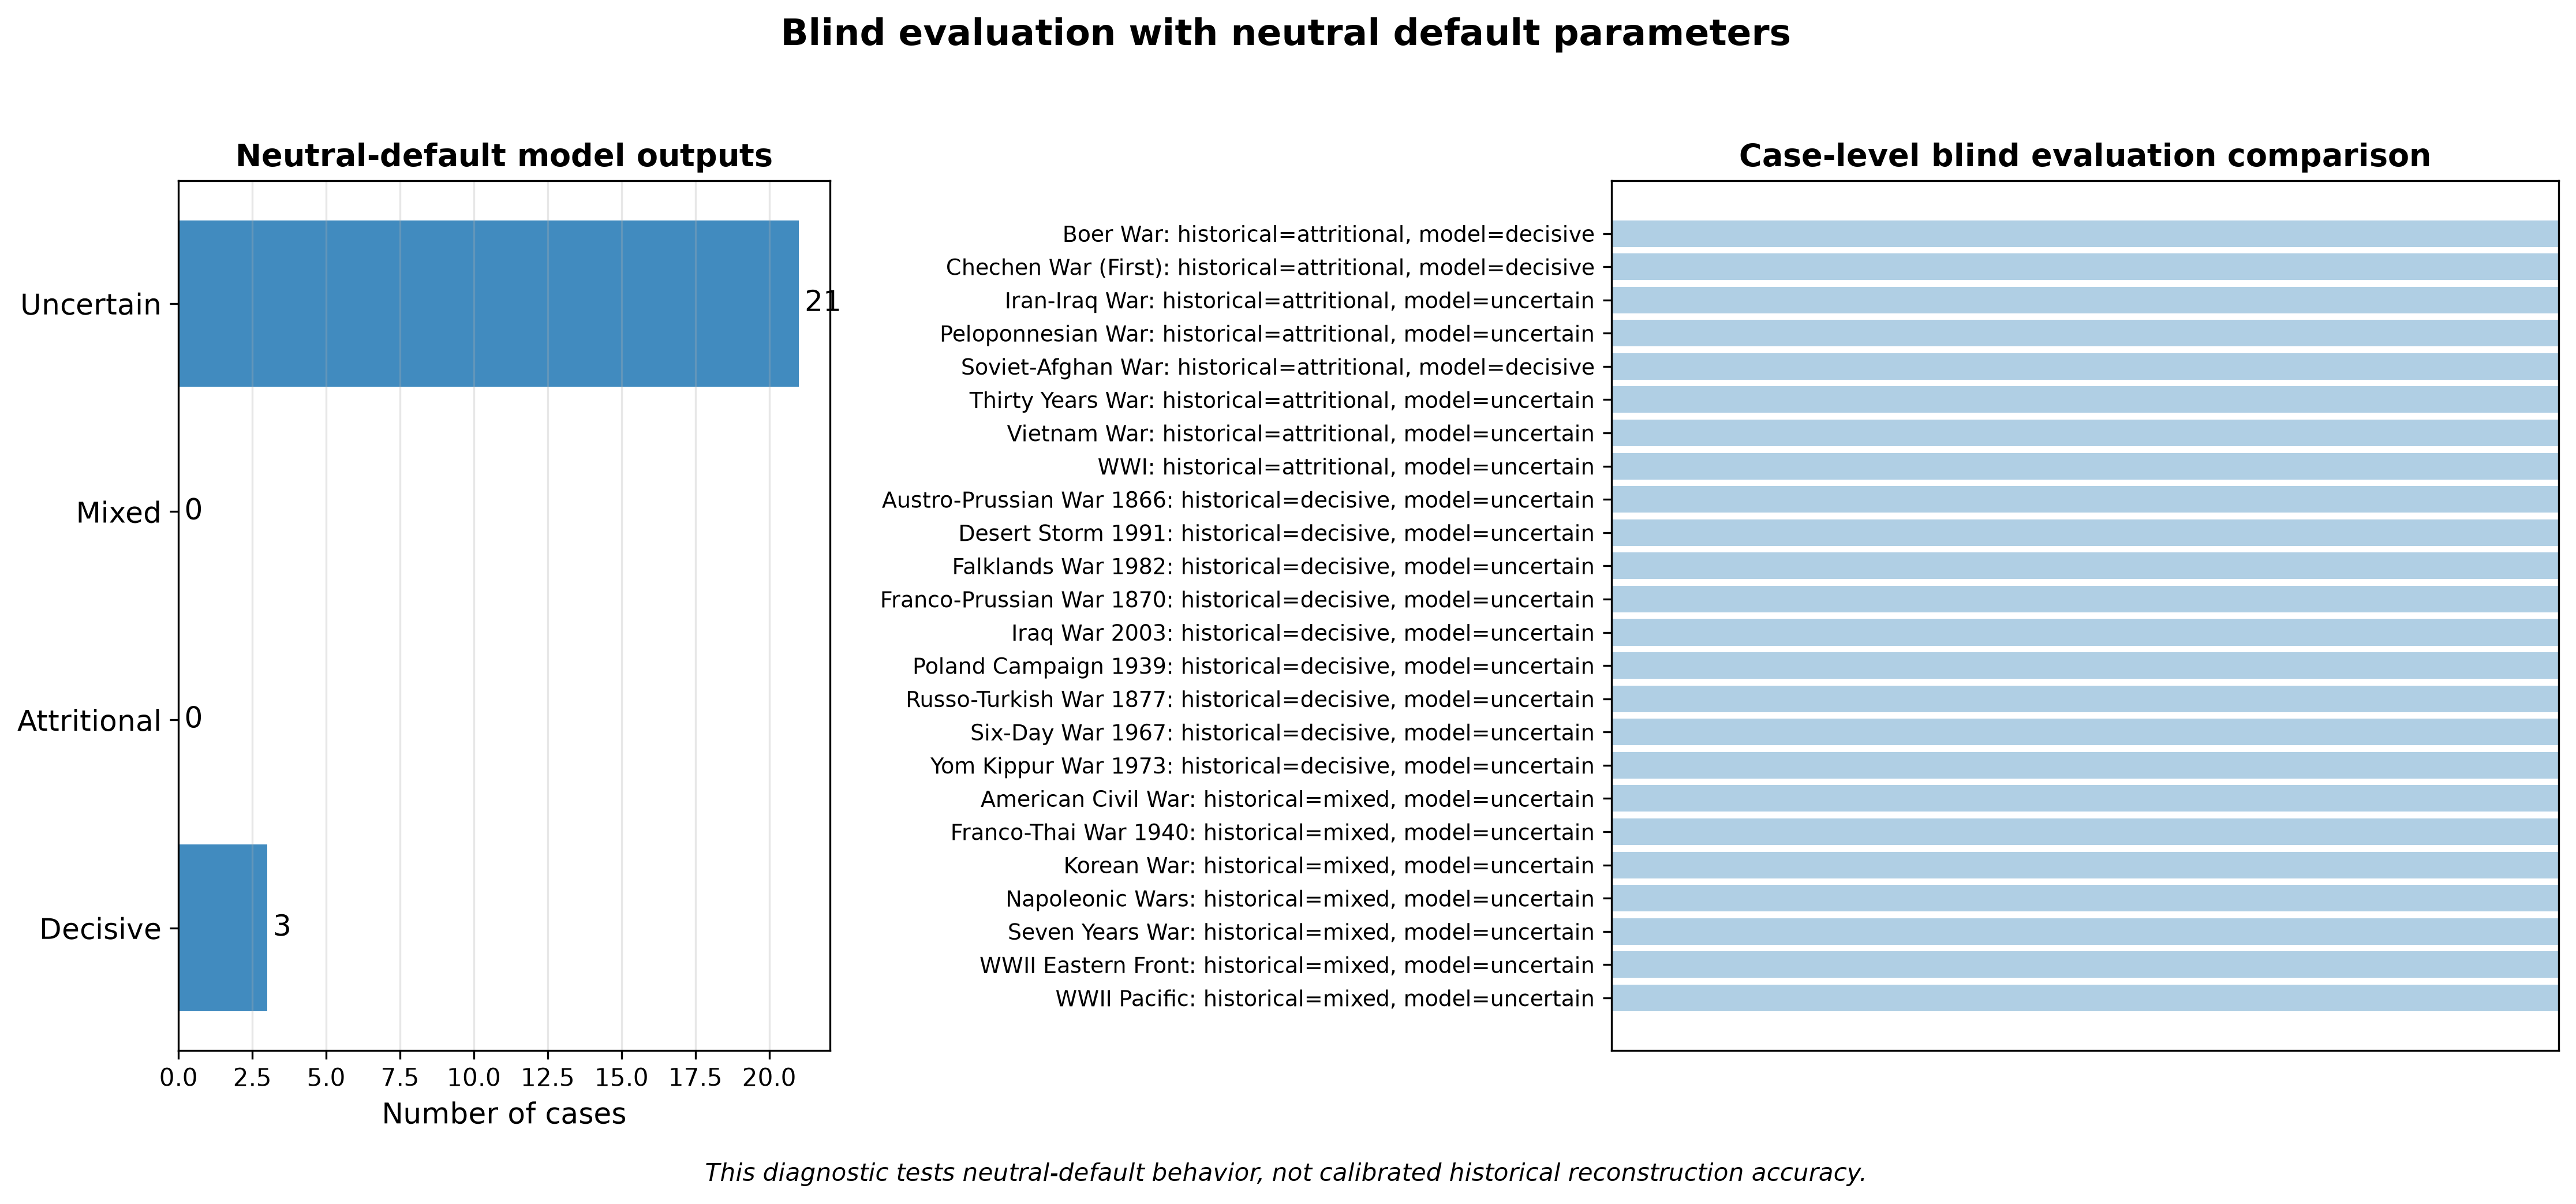
\includegraphics[width=0.8\textwidth]{figures/fig_04_blind_validation.png}
\caption{Blind validation: distribution of preset DSS scores across author-assigned mechanism types (decisive shock, strategic exhaustion, mixed). All cases cluster near the uncertain boundary, confirming that the classifier cannot distinguish mechanisms without case-specific calibration.}
\label{fig:blind_validation}
\end{figure}

\section{ML Model Validation}
\label{app:ml_validation}

The random forest and logistic regression models were validated using 5-fold stratified cross-validation with the following configuration:
\begin{itemize}
    \item Random seed: 42
    \item Cross-validation: Stratified 5-fold
    \item Random forest: 100 trees, max depth 5
    \item Logistic regression: L2 regularization, $C=1.0$, max iterations 2000
    \item Feature scaling: StandardScaler (zero mean, unit variance)
    \item Target: Binary (short war $<$365 days vs.\ long war $\geq$365 days)
    \item Dataset: 2,137 wars with COW National Material Capabilities data
    \item Class balance: 47.7\% short, 52.3\% long
\end{itemize}

The logistic regression achieves 55.0\% $\pm$ 2.2\% cross-validated accuracy (2.7pp above the 52.3\% null baseline), indicating that linear relationships among material-capability features contain limited predictive information. The random forest achieves 72.7\% $\pm$ 1.7\% (AUC = 0.814), indicating that nonlinear interactions among these features contribute substantially to prediction. This 17.7-point gap quantifies the information contained in feature interactions that linear models cannot represent.

\section{Missing Data Severity}
\label{app:missing_data}

Table~\ref{tab:missing_data} quantifies missing data across the seven data sources used in this study. Missing values are imputed to 0 (minimum index contribution), which biases toward uncertainty rather than mechanism classification.

\begin{table}[H]
\centering
\caption{Missing data severity by source and variable. Imputation to 0 reduces index values for incomplete cases.}
\label{tab:missing_data}
\small
\setlength{\tabcolsep}{3pt}
\begin{tabularx}{\textwidth}{@{}>{\RaggedRight\arraybackslash}p{0.22\textwidth} c c >{\RaggedRight\arraybackslash}X@{}}
\toprule
\textbf{Source / Variable} & \textbf{Missing (\%)} & \textbf{Impact} & \textbf{Mitigation} \\
\midrule
\multicolumn{4}{l}{\textit{DSS Components (IWB + Manual)}} \\
\midrule
Casualty concentration & 12\% & High & Imputed to 0; reduces DSS for wars with incomplete battle records \\
Capital capture & 5\% & Low & Binary; missing = no capture \\
Field army destroyed & 8\% & Medium & Binary; missing = not recorded \\
Fleet destroyed & 15\% & Low & Binary; missing = no fleet engagement \\
Rapid surrender & 3\% & Low & Binary; missing = no rapid surrender \\
Regime collapse & 10\% & Medium & Binary; missing = not observed \\
\midrule
\multicolumn{4}{l}{\textit{SES Components (COW + UCDP)}} \\
\midrule
Military expenditure & 22\% & High & Imputed to 0; reduces SES for pre-1949 wars \\
Energy consumption & 35\% & High & Imputed to 0; major gap for pre-SIPRI conflicts \\
Iron \& steel production & 30\% & Medium & Imputed to 0; less critical than energy \\
Battle deaths (annual) & 18\% & Medium & Imputed to 0; reduces cumulative mortality estimate \\
Personnel counts & 15\% & Medium & Imputed to 0; affects manpower depletion metric \\
\midrule
\multicolumn{4}{l}{\textit{Structural DSS Proxy Components}} \\
\midrule
Logistics vulnerability & 100\% & High & Fixed at 50.0; no variation across cases \\
Surprise indicator & 100\% & High & Fixed at 50.0; no variation across cases \\
Alliance asymmetry & 100\% & High & Fixed at 50.0; no variation across cases \\
Mobilization speed & 100\% & High & Fixed at 64.0; no variation across cases \\
Regime stability & 100\% & High & Fixed at 50.0; no variation across cases \\
\bottomrule
\end{tabularx}
\end{table}

\section{Noise Sensitivity}
\label{app:noise_sensitivity}

Table~\ref{tab:noise_sensitivity} reports the results of a Monte Carlo sensitivity analysis with 500 independent noise seeds per historical preset. The noise model adds $\mathcal{N}(0, 0.5)$ to all state variables after each deterministic update step.

\begin{table}[H]
\centering
\caption{Noise sensitivity across 500 seeds per historical preset. Dominant share is the fraction of runs producing the most common termination outcome.}
\label{tab:noise_sensitivity}
\small
\begin{tabularx}{\textwidth}{@{}>{\RaggedRight\arraybackslash}X l c c c c c@{}}
\toprule
\textbf{Case} & \textbf{Dominant outcome} & \textbf{Share} & \textbf{Min} & \textbf{Median} & \textbf{Max} & \textbf{Outcomes} \\
\midrule
Gulf War 1991 & dominance\_a & 1.00 & 13 & 18 & 24 & 1 \\
Vietnam War & withdrawal\_a & 0.79 & 63 & 90 & 124 & 2 \\
Wwi & exhaustion\_b & 0.62 & 54 & 65 & 76 & 2 \\
Franco Prussian & dominance\_a & 1.00 & 9 & 12 & 18 & 1 \\
Korean War & negotiated\_settlement & 1.00 & 40 & 44 & 49 & 1 \\
Iran Iraq & mutual\_exhaustion & 0.97 & 69 & 83 & 102 & 2 \\
Wwii & mutual\_exhaustion & 0.77 & 58 & 68 & 78 & 2 \\
\bottomrule
\end{tabularx}
\end{table}


Three cases show non-trivial noise sensitivity: World War I (62\% dominant share), World War II (77\% dominant share), and the Vietnam War (79\% dominant share). These cases produce two distinct termination outcomes across 500 runs, indicating that the classification boundary is sensitive to stochastic perturbation. The remaining four cases (Gulf War, Franco-Prussian War, Korean War, Iran--Iraq) are highly stable with dominant shares of 97--100\%. The noise-sensitive cases should be interpreted with appropriate caution: their mechanism classifications are probabilistic rather than deterministic.

\section{Statistical Model Audit}
\label{app:statistical_audit}

Table~\ref{tab:statistical_audit} reports the full statistical model audit including variance inflation factors, out-of-bag error, interaction logistic regression, and bootstrap confidence intervals.

\begin{table}[H]
\centering
\caption{Statistical model audit: VIF, out-of-bag error, interaction logistic regression, and bootstrap AUC confidence intervals.}
\label{tab:statistical_audit}
\small
\setlength{\tabcolsep}{4pt}
\begin{tabularx}{\textwidth}{@{}l X r@{}}
\toprule
\textbf{Metric} & \textbf{Details} & \textbf{Value} \\
\midrule
\multicolumn{3}{l}{\textit{Variance Inflation Factors}} \\
energy consumption initial & High & 36.05 \\
cinc pct change & High & 21.79 \\
iron steel initial & High & 18.48 \\
military personnel pct change & High & 16.40 \\
military expenditure initial & Warning & 8.14 \\
military expenditure pct change & OK & 4.56 \\
energy consumption pct change & OK & 4.28 \\
iron steel pct change & OK & 4.11 \\
cinc initial & OK & 3.08 \\
battle deaths initial & OK & 2.49 \\
military personnel initial & OK & 2.18 \\
battle deaths pct change & OK & 1.05 \\
\midrule
\multicolumn{2}{l}{\textbf{Max VIF}} & 36.05 \\
\midrule
\multicolumn{3}{l}{\textit{Model Performance}} \\
Logistic regression test accuracy & 5-fold CV, $C=1.0$ & 0.5483 \\
Logistic regression AUC-ROC & Bootstrap 95\% CI & 0.5610 \\
  LR AUC 95\% CI & $[0.5165,\; 0.6048]$ & \\
Interaction logistic test accuracy & Degree-2 interactions, L2 & 0.5935 \\
Interaction logistic AUC-ROC & & 0.6293 \\
Random forest test accuracy & 100 trees, depth 5 & 0.7321 \\
Random forest AUC-ROC & Bootstrap 95\% CI & 0.7946 \\
  RF AUC 95\% CI & $[0.7598,\; 0.8282]$ & \\
Random forest OOB accuracy & Out-of-bag estimate & 0.7358 \\
\bottomrule
\end{tabularx}
\end{table}


The maximum VIF of 36.05 (energy consumption initial) indicates substantial multicollinearity among the initial-condition features. This is expected: countries with high energy consumption also tend to have high CINC scores, military expenditure, and iron/steel production. The random forest is robust to multicollinearity, but the logistic regression coefficients should be interpreted with caution. The interaction logistic regression (AUC 0.63) provides modest improvement over the baseline logistic (AUC 0.56), while the random forest (AUC 0.79) captures substantially more nonlinear structure. The 95\% bootstrap confidence intervals confirm that the random forest's AUC advantage over logistic regression is statistically significant (non-overlapping intervals).

\section{Empirical vs.\ Simulation Traceability}
\label{app:traceability}

Table~\ref{tab:traceability} maps each claim in the main text to its source: empirical (computed from external data), simulation (computed from model trajectories), or mixed (empirical data fed into simulation). This traceability prevents the conflation of data-derived findings with simulation-generated outputs.

\begin{table}[H]
\centering
\caption{Empirical vs.\ simulation traceability. Each major finding is traced to its data source.}
\label{tab:traceability}
\small
\setlength{\tabcolsep}{3pt}
\begin{tabularx}{\textwidth}{@{}>{\RaggedRight\arraybackslash}p{0.32\textwidth} >{\centering\arraybackslash}p{0.14\textwidth} >{\RaggedRight\arraybackslash}X@{}}
\toprule
\textbf{Finding} & \textbf{Source} & \textbf{Details} \\
\midrule
4,812 wars total & Empirical & Merged COW + Brecke + UCDP datasets \\
91 wars with battle data & Empirical & Interstate War Battle Dataset subset \\
2.2\% decisive shock & Empirical & DSS computed from IWB battle-level data \\
22.0\% strategic exhaustion & Empirical & SES computed from war-year COW data \\
75.8\% uncertain & Empirical & DSS--SES difference $<$ 20 in both directions \\
6/7 mechanism agreement & Mixed & Simulation trajectories compared to author-assigned labels \\
72.7\% RF accuracy & Empirical & Trained on COW NMC features only \\
55.0\% LR accuracy & Empirical & Same features, linear baseline \\
Parameter sensitivity (0.3\% flip) & Simulation & 23 internal coefficients varied $\pm 50\%$ \\
Threshold sensitivity (86.1\% mean) & Simulation & 175 parameter combinations \\
Gulf War = decisive & Mixed & Simulation trajectory consistent with author-assigned label \\
Vietnam = exhaustion & Mixed & Simulation trajectory consistent with author-assigned label \\
Attritional iceberg pattern & Empirical & Distribution of DSS/SES across 91 wars \\
\bottomrule
\end{tabularx}
\end{table}

\section*{Supplementary Materials}

\subsection*{S1. Capability Transitions}

Figure~\ref{fig:trajectory_examples} shows start-to-end aggregate CINC transitions for five selected COW conflicts. Each row aggregates participant capability within the first and last observed conflict years, then reports the direction and magnitude of the capability change.

\begin{figure}[H]
\centering
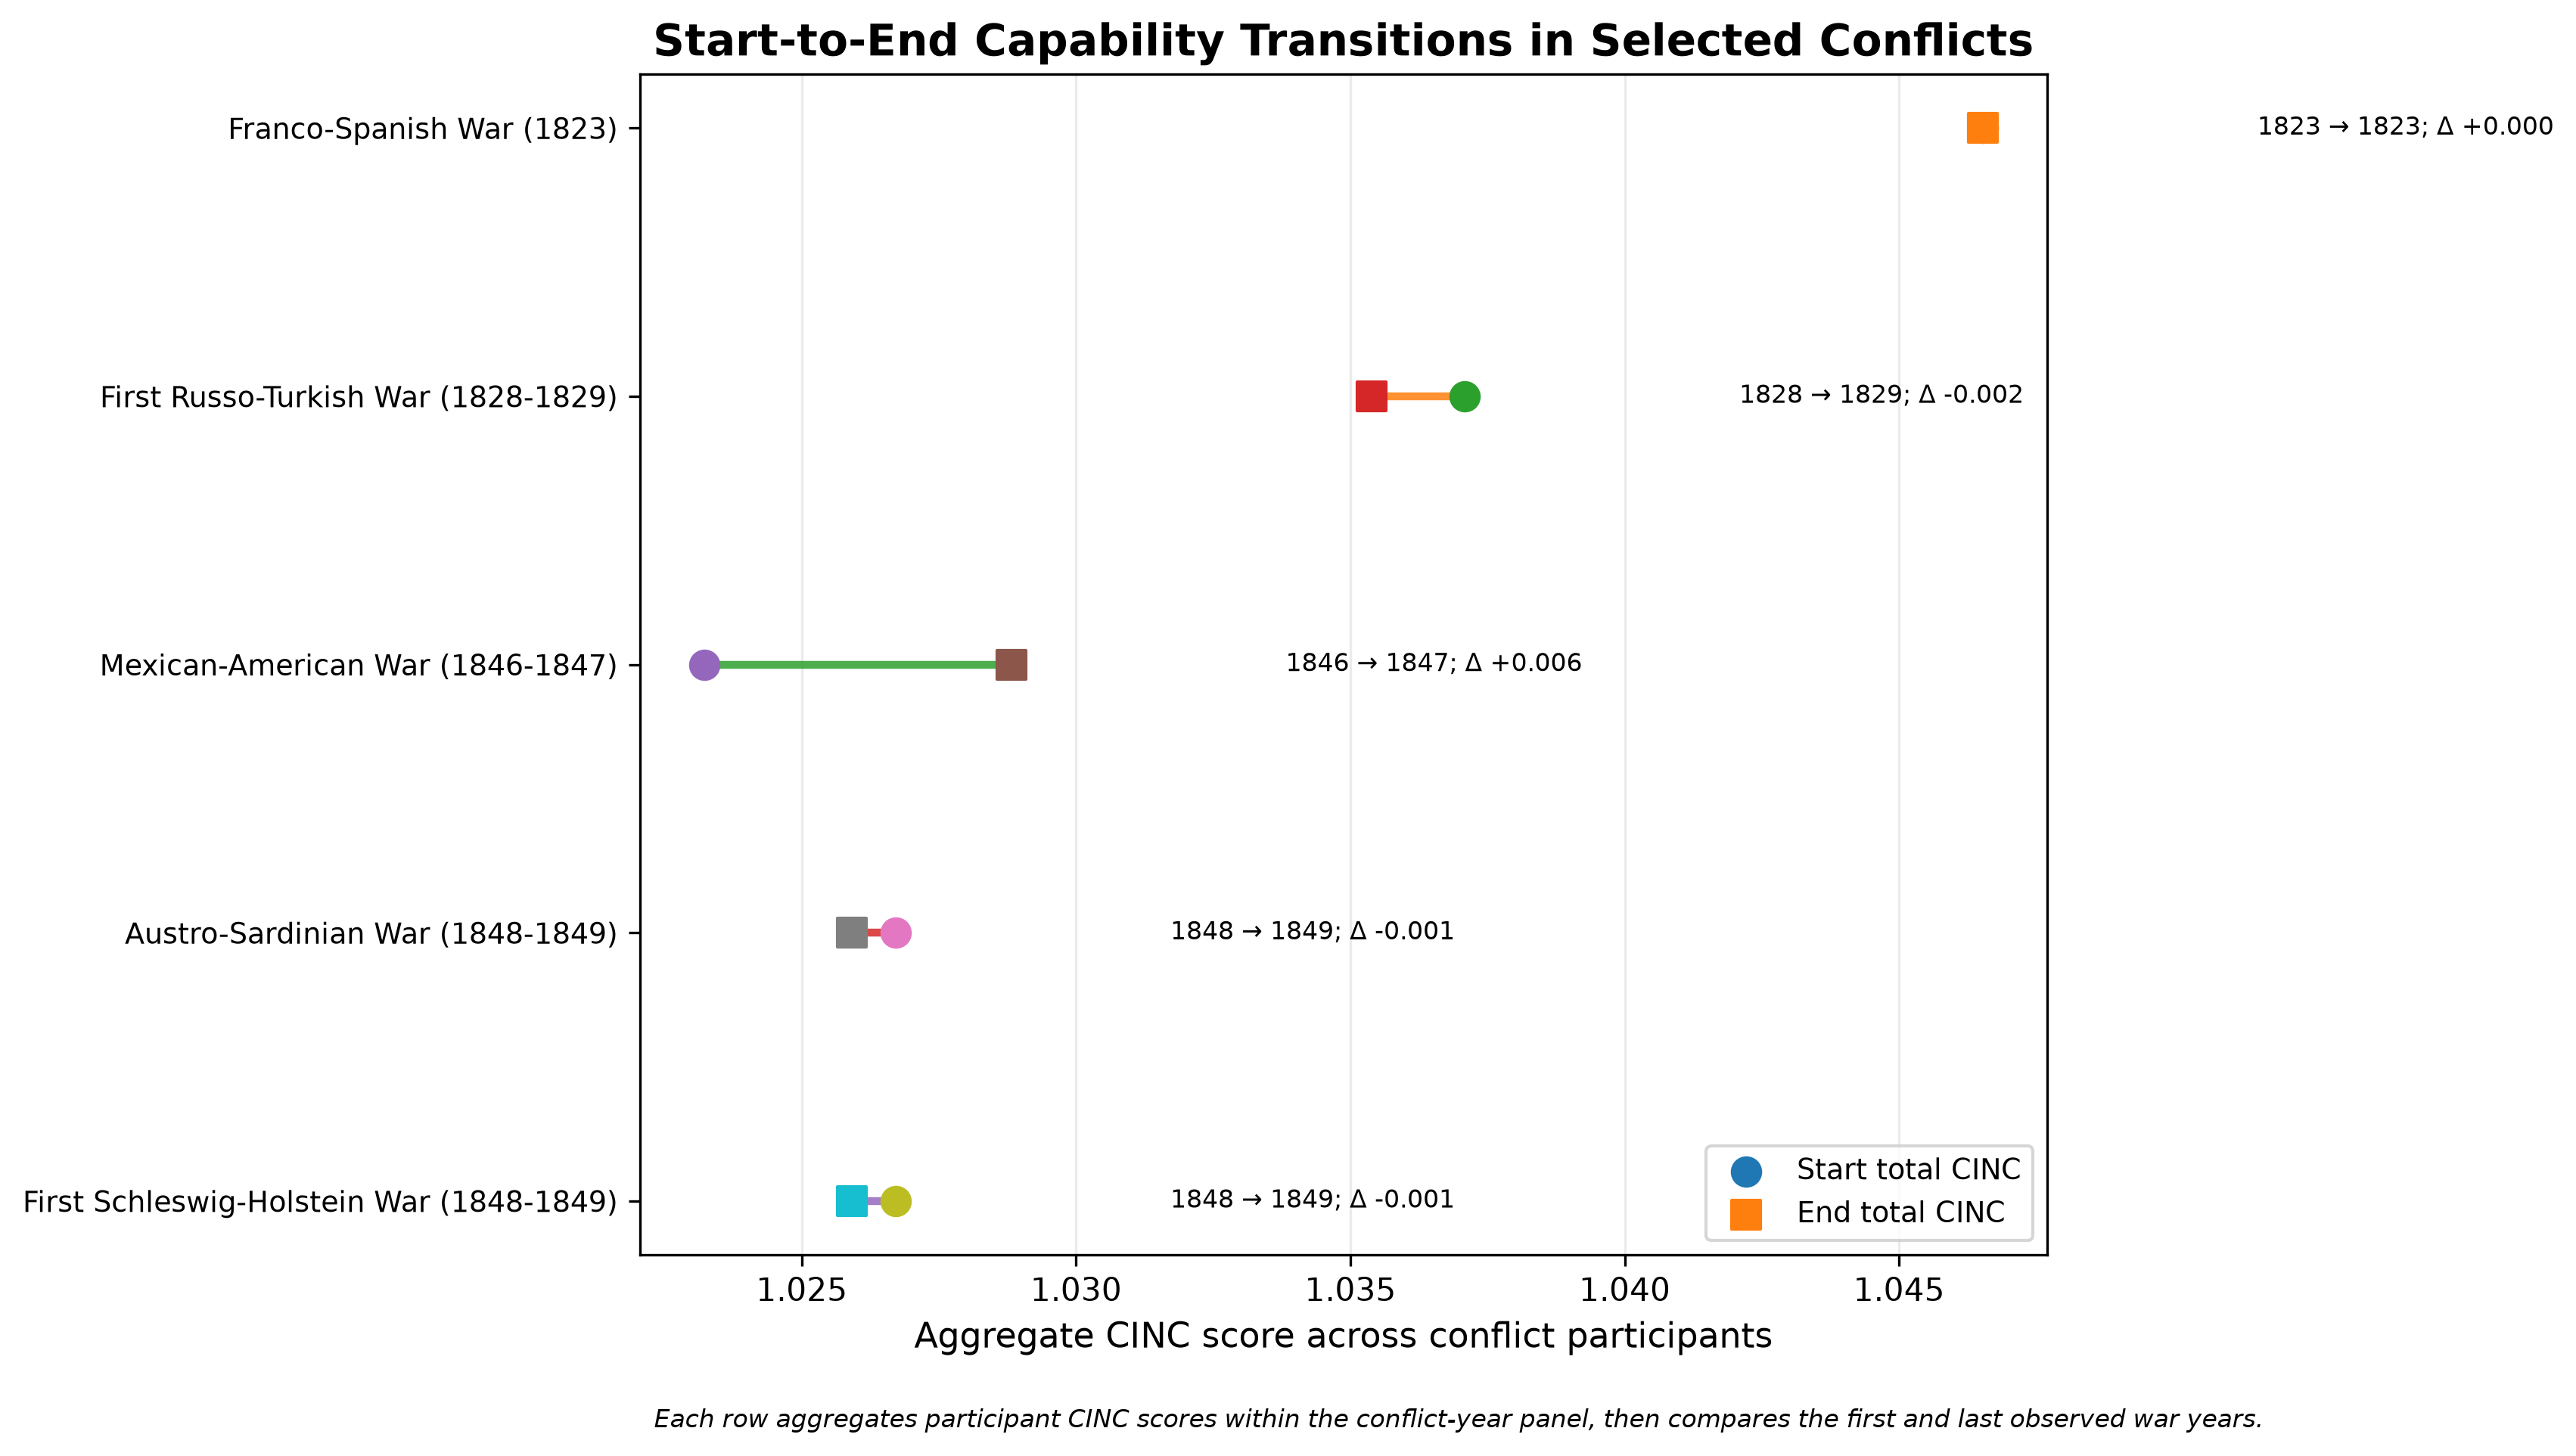
\includegraphics[width=0.65\textwidth]{figures/fig_06_trajectory_examples.png}
\caption{Start-to-end aggregate capability transitions for five selected conflicts. Circles mark the first observed conflict year, squares mark the last observed conflict year, and annotations report the year span and aggregate CINC change.}
\label{fig:trajectory_examples}
\end{figure}

\subsection*{S2. Historical Case Scorecards}

Figure~\ref{fig:case_study_scorecards} presents historical case-study DSS and SES scorecards. The bars show manually assigned historical interpretation scores used for structured comparison; they are not separate model predictions.

\begin{figure}[H]
\centering
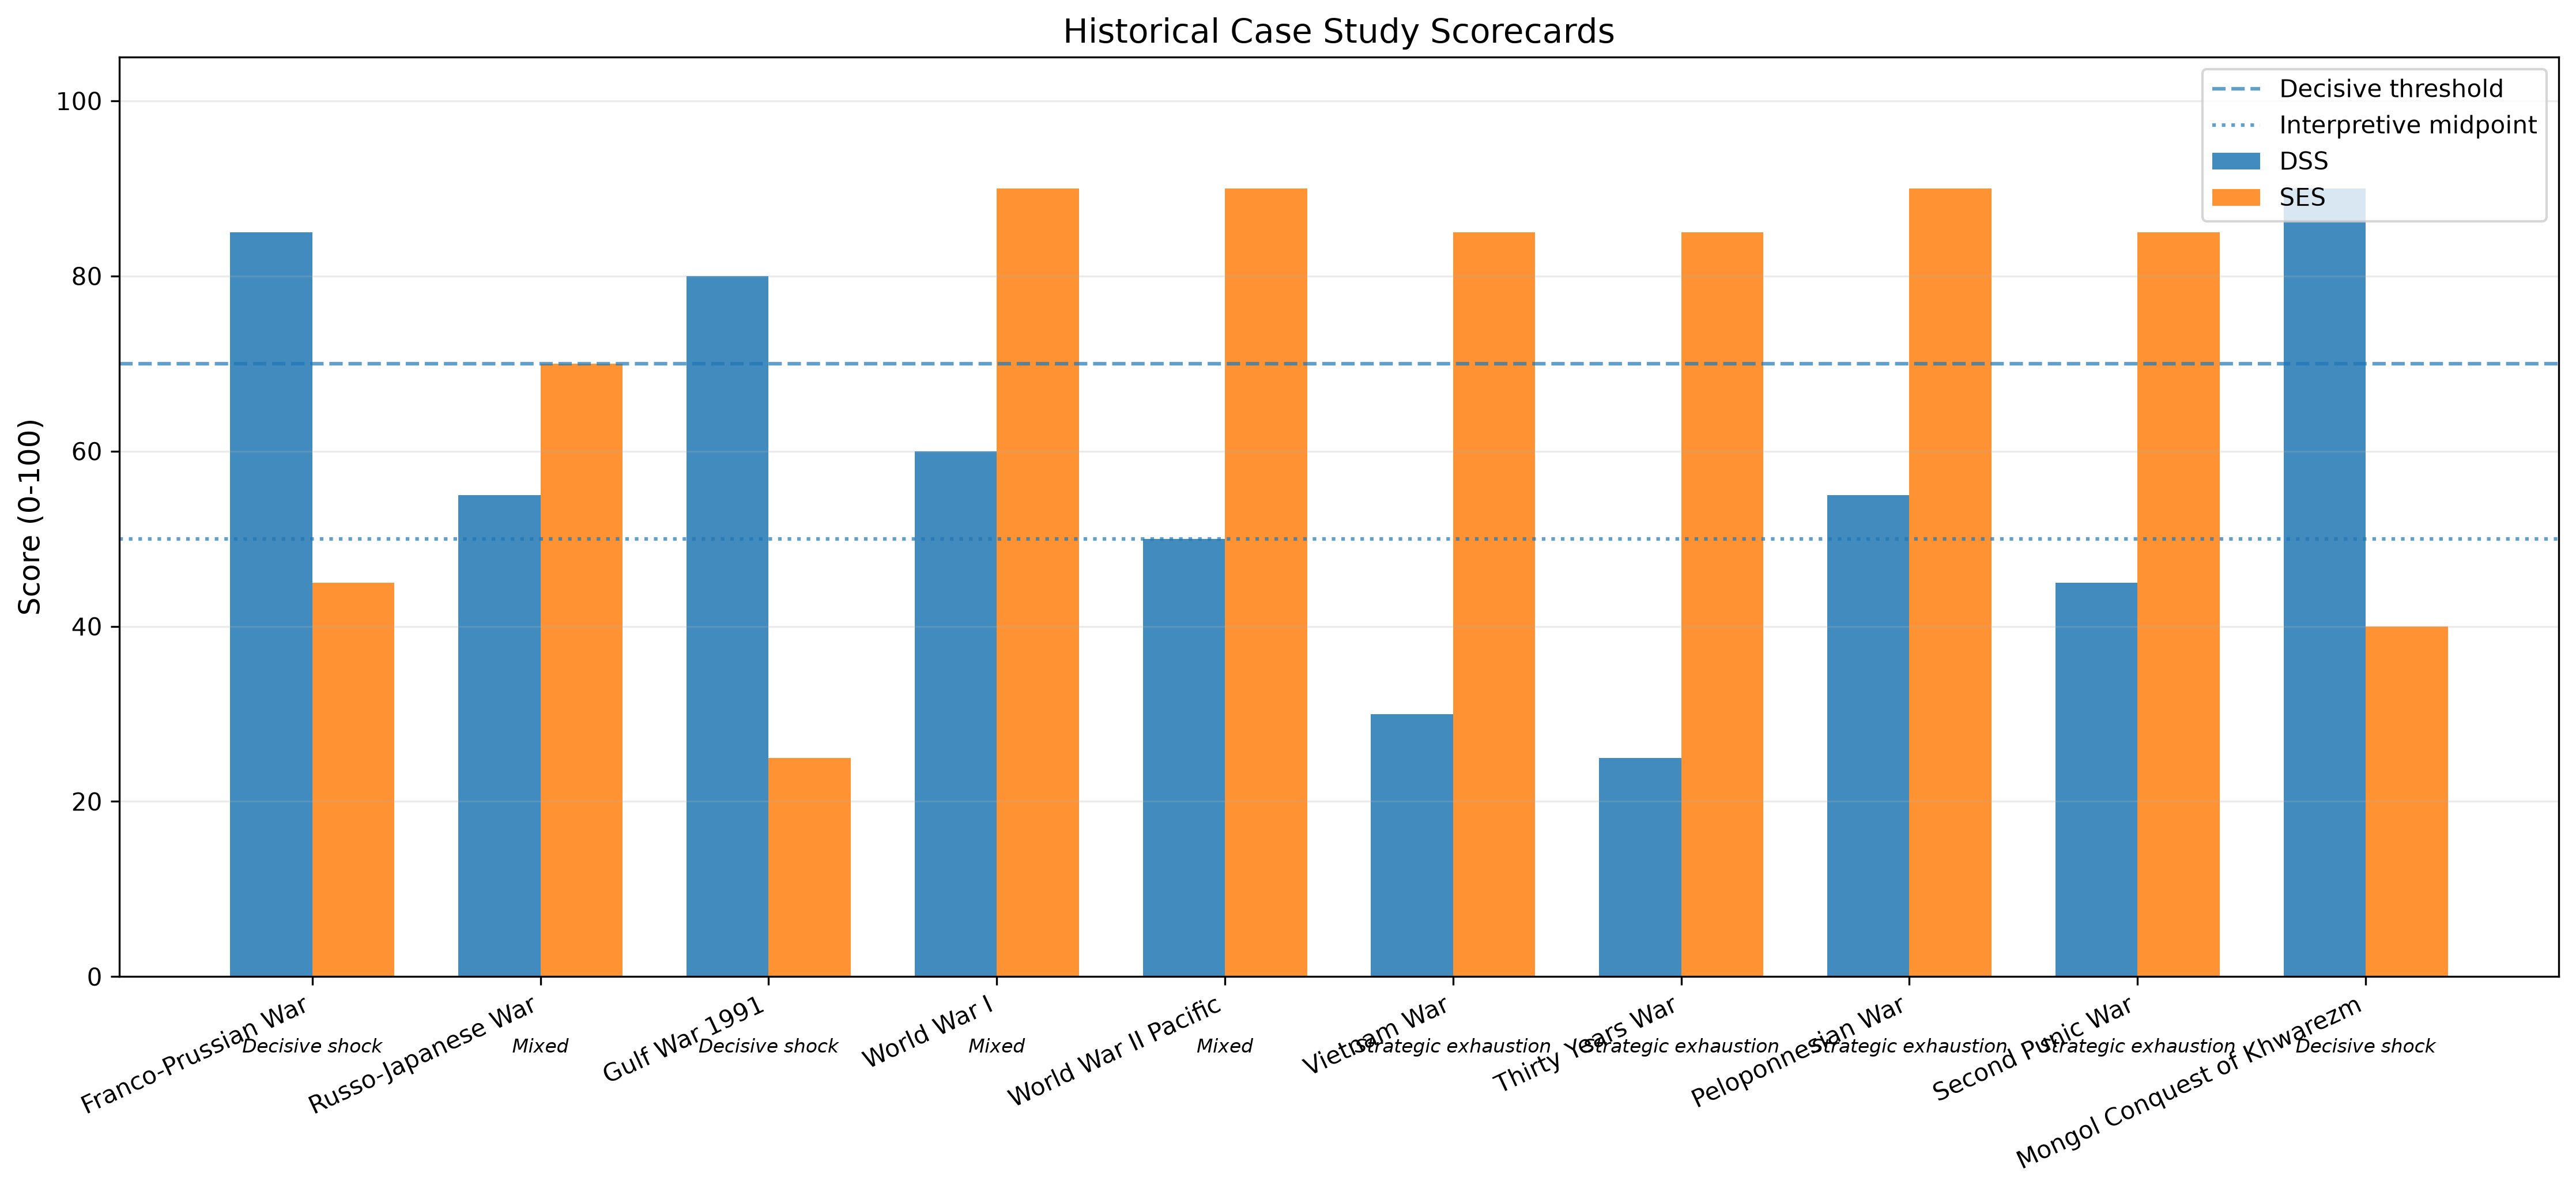
\includegraphics[width=0.65\textwidth]{figures/fig_07_case_study_scorecards.png}
\caption{Historical case-study scorecards. Bars show DSS and SES interpretation scores for selected conflicts.}
\label{fig:case_study_scorecards}
\end{figure}


\end{document}
